  \documentclass[a4paper, 11pt, titlepage]{article}
\usepackage[a4paper,top=2.25cm,bottom=2.25cm,left=2cm,right=2cm,marginparwidth=2cm]{geometry}
\usepackage{amsmath}
\usepackage{graphicx}
\usepackage[toc,page]{appendix}
\usepackage[colorlinks=true, allcolors=blue]{hyperref}
\usepackage{caption}
\usepackage{titlepic}
\usepackage{titling}
\usepackage{wrapfig}
\usepackage{stfloats}
\usepackage{placeins}
\usepackage[urldate=iso,seconds=true]{biblatex} %Imports biblatex package
\addbibresource{sample.bib} %Import the bibliography file
\usepackage[english,serbian]{babel}
\usepackage{framed}
\usepackage[dvipsnames]{xcolor}
\usepackage{tcolorbox}
\usepackage{listings}
\usepackage{xcolor}
\usepackage{pdfcomment}
\usepackage{enumitem}
\usepackage{multirow}
\definecolor{beaublue}{rgb}{0.74, 0.83, 0.9}
\definecolor{babyblueeyes}{rgb}{0.63, 0.79, 0.95}
\definecolor{codegreen}{rgb}{0,0.6,0}
\definecolor{codegray}{rgb}{0.5,0.5,0.5}
\definecolor{codepurple}{rgb}{0.58,0,0.82}
\definecolor{backcolour}{rgb}{0.95,0.95,0.92}

\lstdefinestyle{mystyle}{
    backgroundcolor=\color{backcolour},   
    commentstyle=\color{codegreen},
    keywordstyle=\color{magenta},
    numberstyle=\tiny\color{codegray},
    stringstyle=\color{codepurple},
    basicstyle=\ttfamily\footnotesize,
    breakatwhitespace=false,         
    breaklines=true,                 
    captionpos=b,                    
    keepspaces=true,                 
    numbers=left,                    
    numbersep=5pt,                  
    showspaces=false,                
    showstringspaces=false,
    showtabs=false,                  
    tabsize=2
}

\lstset{style=mystyle}

\def\departman{Departman za računarstvo i automatiku}
\def\odsek{Odsek za računarsku tehniku i računarske komunikacije}
\def\reporttitle{Diesel generator} 
\def\institutionname{UNIVERZITET U NOVOM SADU}
\def\institutionnames{FAKULTET TEHNIČKIH NAUKA}
\def\cityname{NOVI SAD}
\def\authornameA{Kandidat: Nikola Bošković RA 39/2021} 
\def\authornameB{Kandidat: Vuk Antović RA 52/2021} 
\def\authornameC{Kandidat: Ana Mujić RA 58/2021} 
\def\authornameD{Kandidat: Ante Rešetar RA 61/2021} 
\def\authornameE{Kandidat: Aleksandar Ivanović RA 79/2021} 

\def\predmet{Predmet: Logičko projektovanje računarskih sistema 2}
\def\mentor{Mentori rada: dr Miloš Subotić i Aleksandar Petrovski}
\title{\reporttitle}
\def\reportsubtitle{air flow, t - sensors and throttle-by-wire}
\def\reportsubtitleA{projektni zadatak}

\date{\today}

\usepackage{fancyhdr}
\pagestyle{fancy}
\fancyhf{}
\lhead{\reporttitle}
\setlength{\headheight}{13.6pt}
\addtolength{\topmargin}{-1.6pt}
\rfoot{\thepage}

\begin{document}
\begin{titlepage} 
\newcommand{\HRule}{\rule{\linewidth}{0.5mm}}

\center
\textsc{\Large \institutionname}\\[0.2cm]
\textsc{\Large \institutionnames}\\[0.2cm]
\textsc{\Large \cityname}\\[0.2cm]
\textmd{\Large \departman}\\[0.1cm] 
\textmd{\Large \odsek}\\[0.1cm] 


\HRule\\[0.8cm]

{\Huge\bfseries \reporttitle}\\[0.4cm]
\else
{\textsc{\huge \reportsubtitleA}}\\[0.4cm] 
\fi
\HRule\\[1.5cm]

\authornameA \\[0.5cm]
\authornameB \\[0.5cm]
\authornameC \\[0.5cm]
\authornameD \\[0.5cm]
\authornameE \\[0.5cm]


\predmet\\[0.5cm]
\mentor \\[0.5cm]

\vfill\vfill\vfill\vfill\vfill\vfill\vfill\vfill\vfill\vfill\vfill\vfill\vfill\vfill\vfill\vfill\vfill\vfill\vfill\vfill\vfill

{\large Novi Sad, letnji semestar 2024.}

%\includegraphics[width=0.2\textwidth]{images/qut-logo.jpg}\\[1cm] % Include a department/university logo - this will require the graphicx package
 
\end{titlepage}
% \maketitle
{\hypersetup{linkcolor=black} 
% \let\clearpage\relax 
\thispagestyle{empty}
\newpage
\thispagestyle{empty}
\tableofcontents
\newpage

\pagenumbering{arabic}
}

\newpage
\section{Opis zadatka}
\rhead{Opis zadatka}


Zadatak ovog projekta je istraživanje datog dizel motora. \\
Dizel motor je bilo potrebno popraviti, nacrtati šemu motora i njegove elektronike za dalji rad, kao i poboljšanje njegove funkcionalnosti time što je omogućeno njegovo ukljčivanje na dugme i potenciometar umesto ključa i menjača.



\newpage
\section{Hronološki tok projekta}
\rhead{Hronološki tok projekta}

Prva stvar koju smo uradili jeste da smo očistili generator i istraživali koje napajanje mu je potrebno da bismo ga pokrenuli. 
Kako je vukao poprilično struje, istražili smo i nabavili akumulator koji mu je potreban. Takođe, zamenili smo crevo koje dovodi gorivo iz rezervoara u motor. \\

\begin{figure}[htbp]
  \centering
  \begin{minipage}[b]{0.3\textwidth}
    \centering
    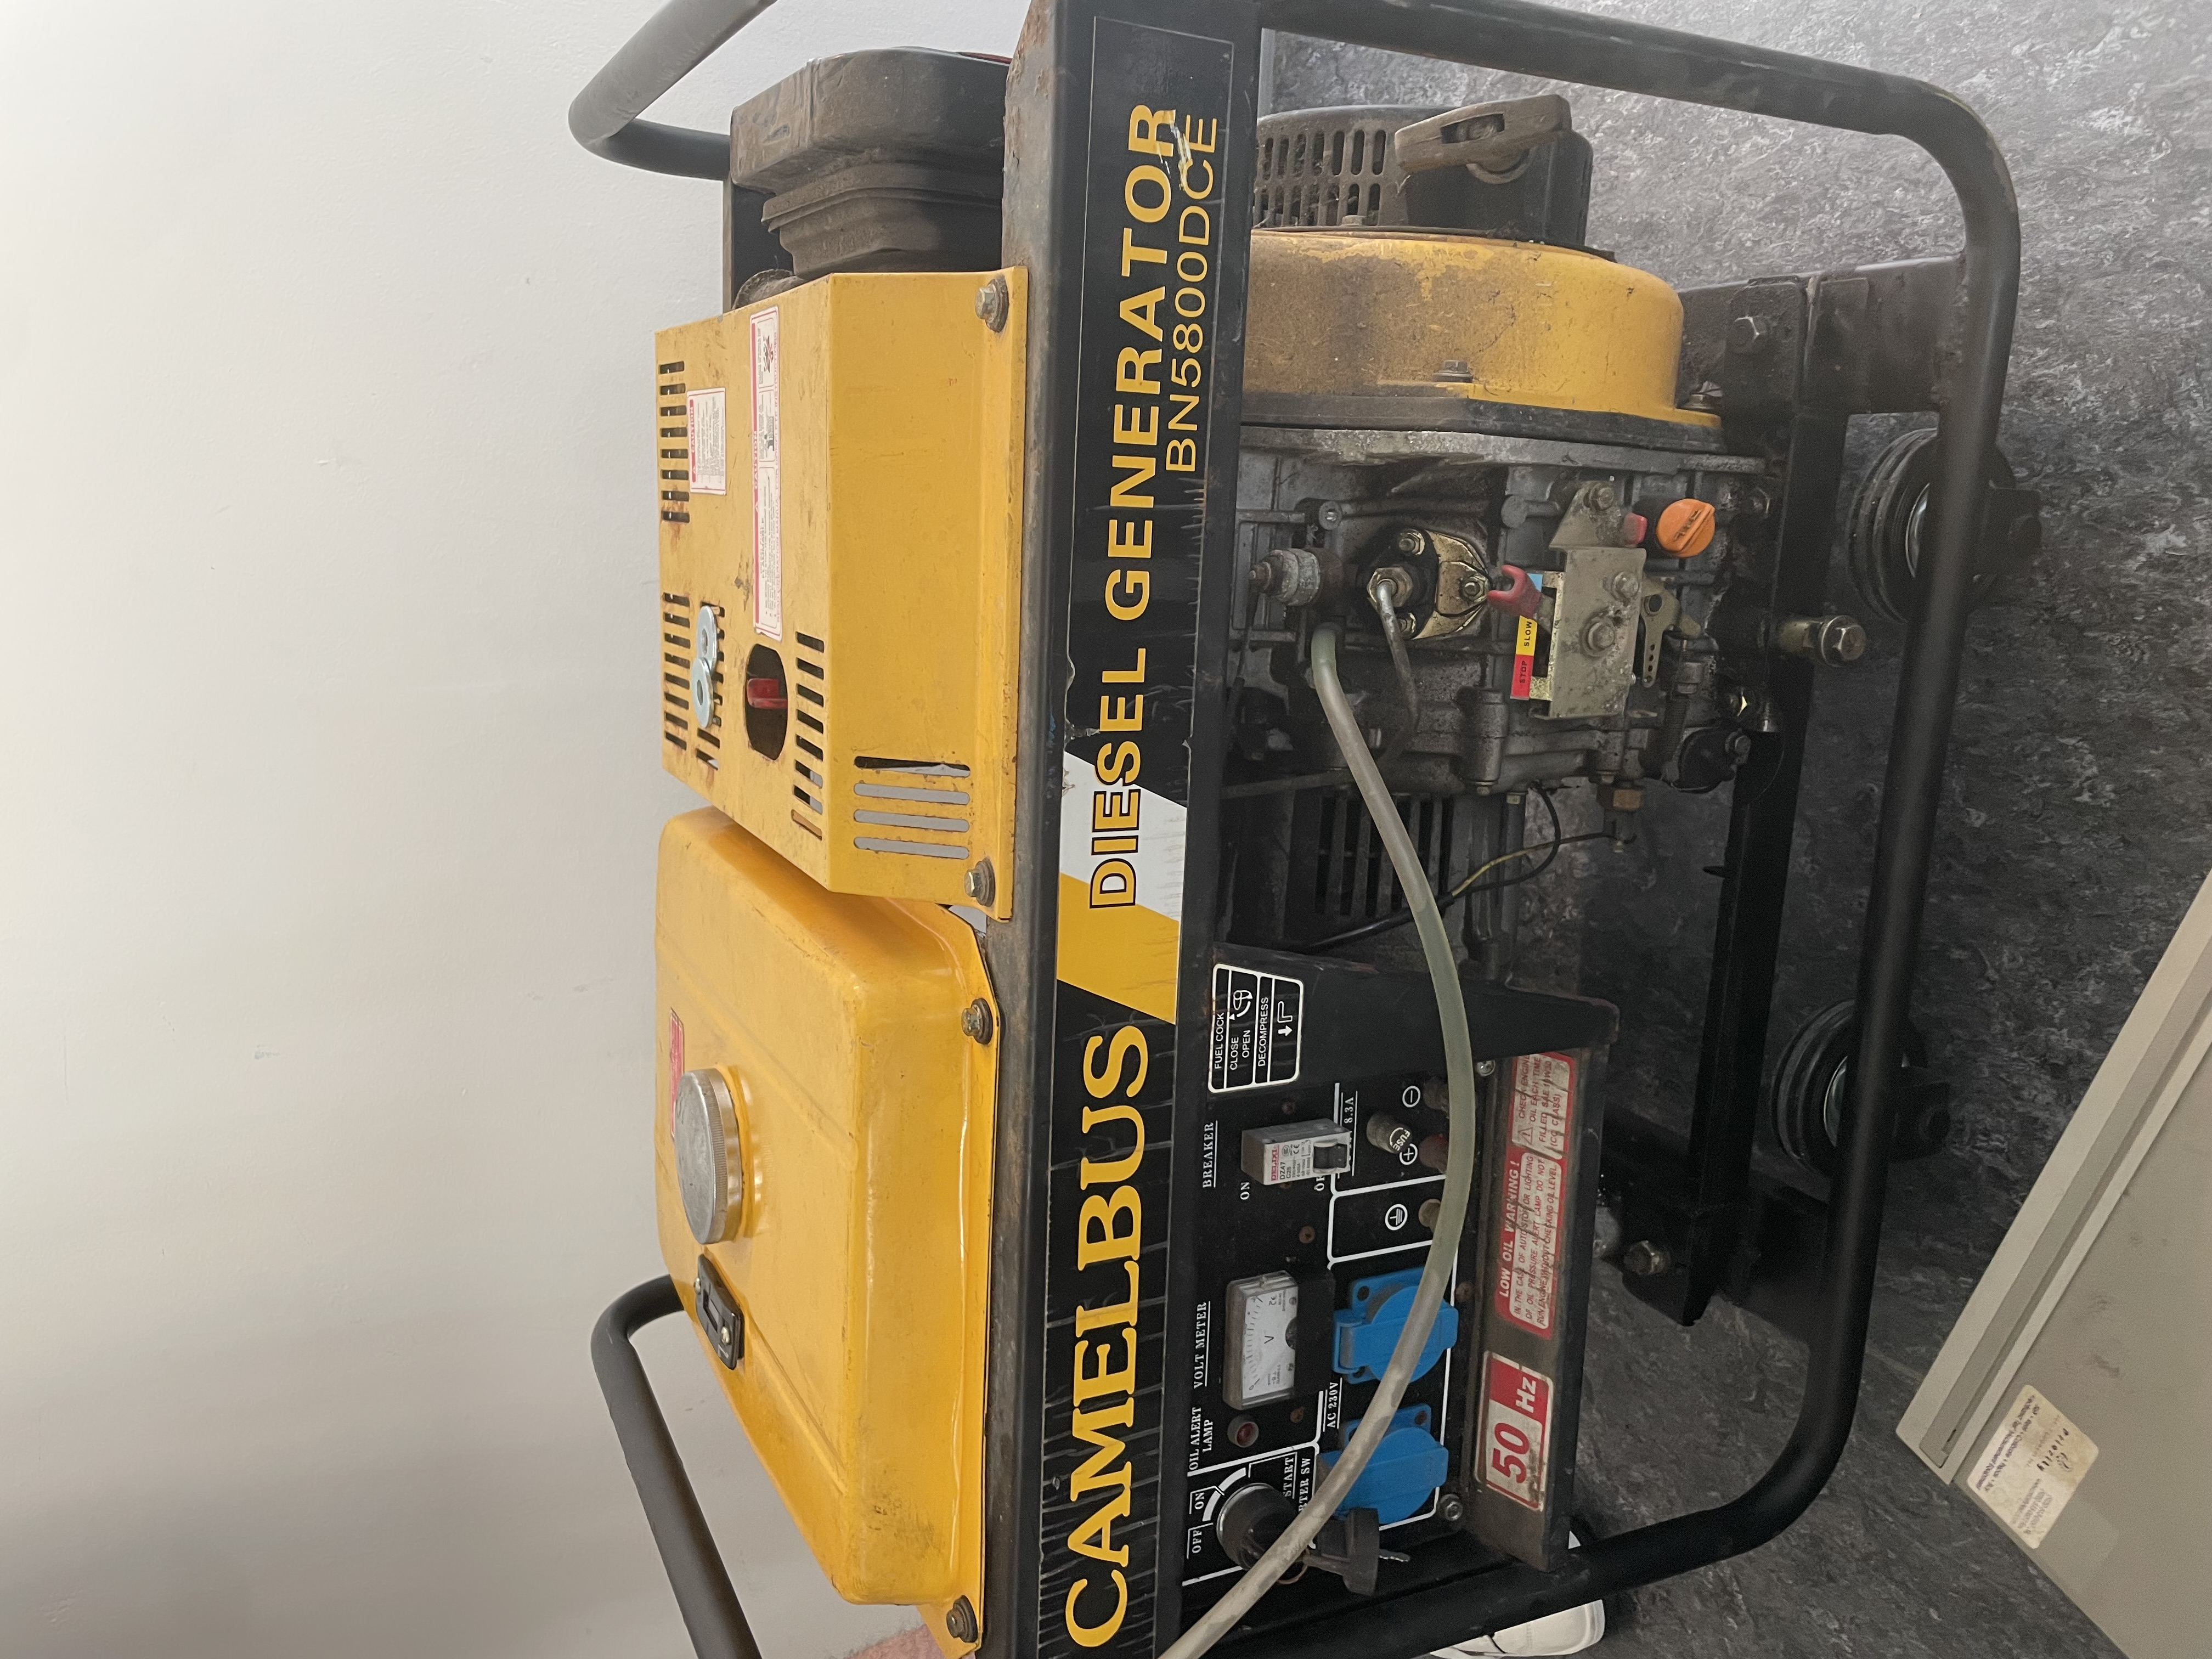
\includegraphics[angle = 270, width=0.75\linewidth]{IMG_4276.png}
    \caption{Dizel generator}
  \end{minipage}
  \hfill
  \begin{minipage}[b]{0.3\textwidth}
    \centering
    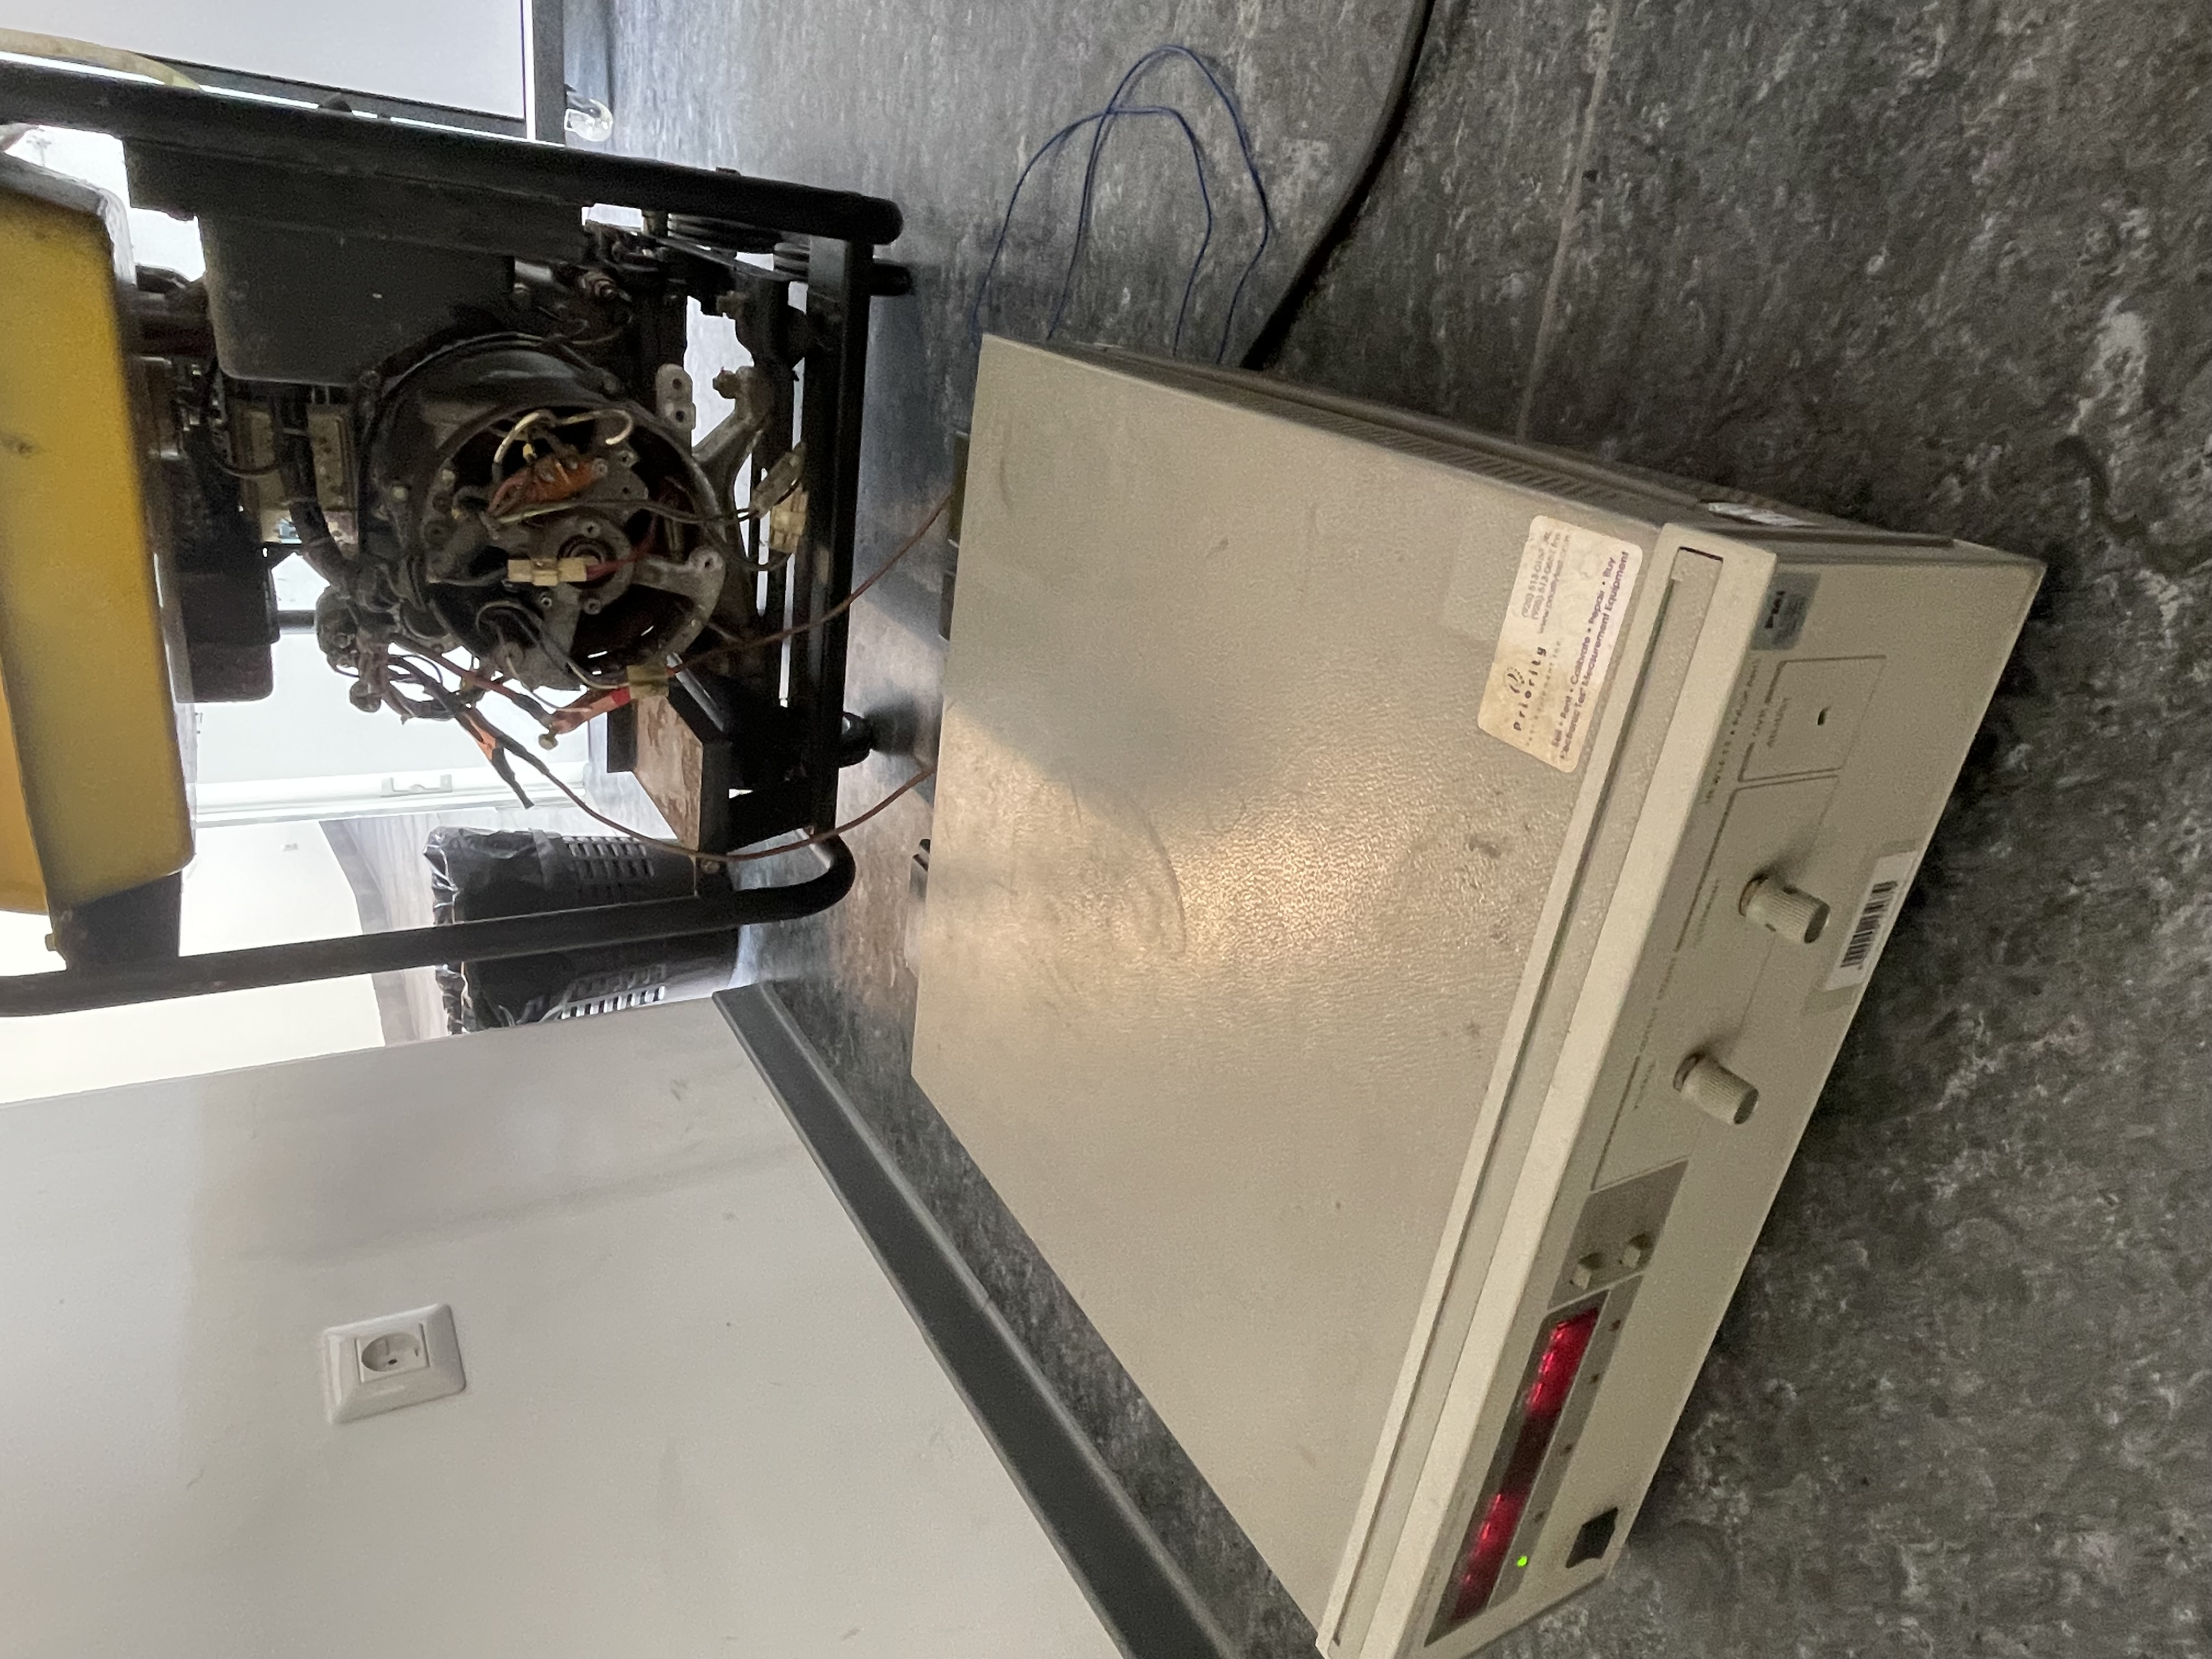
\includegraphics[angle = 270, width=0.75\linewidth]{IMG_4280.jpeg}
    \caption{Merenje napajanja}
  \end{minipage}
    \hfill
  \begin{minipage}[b]{0.3\textwidth}
    \centering
    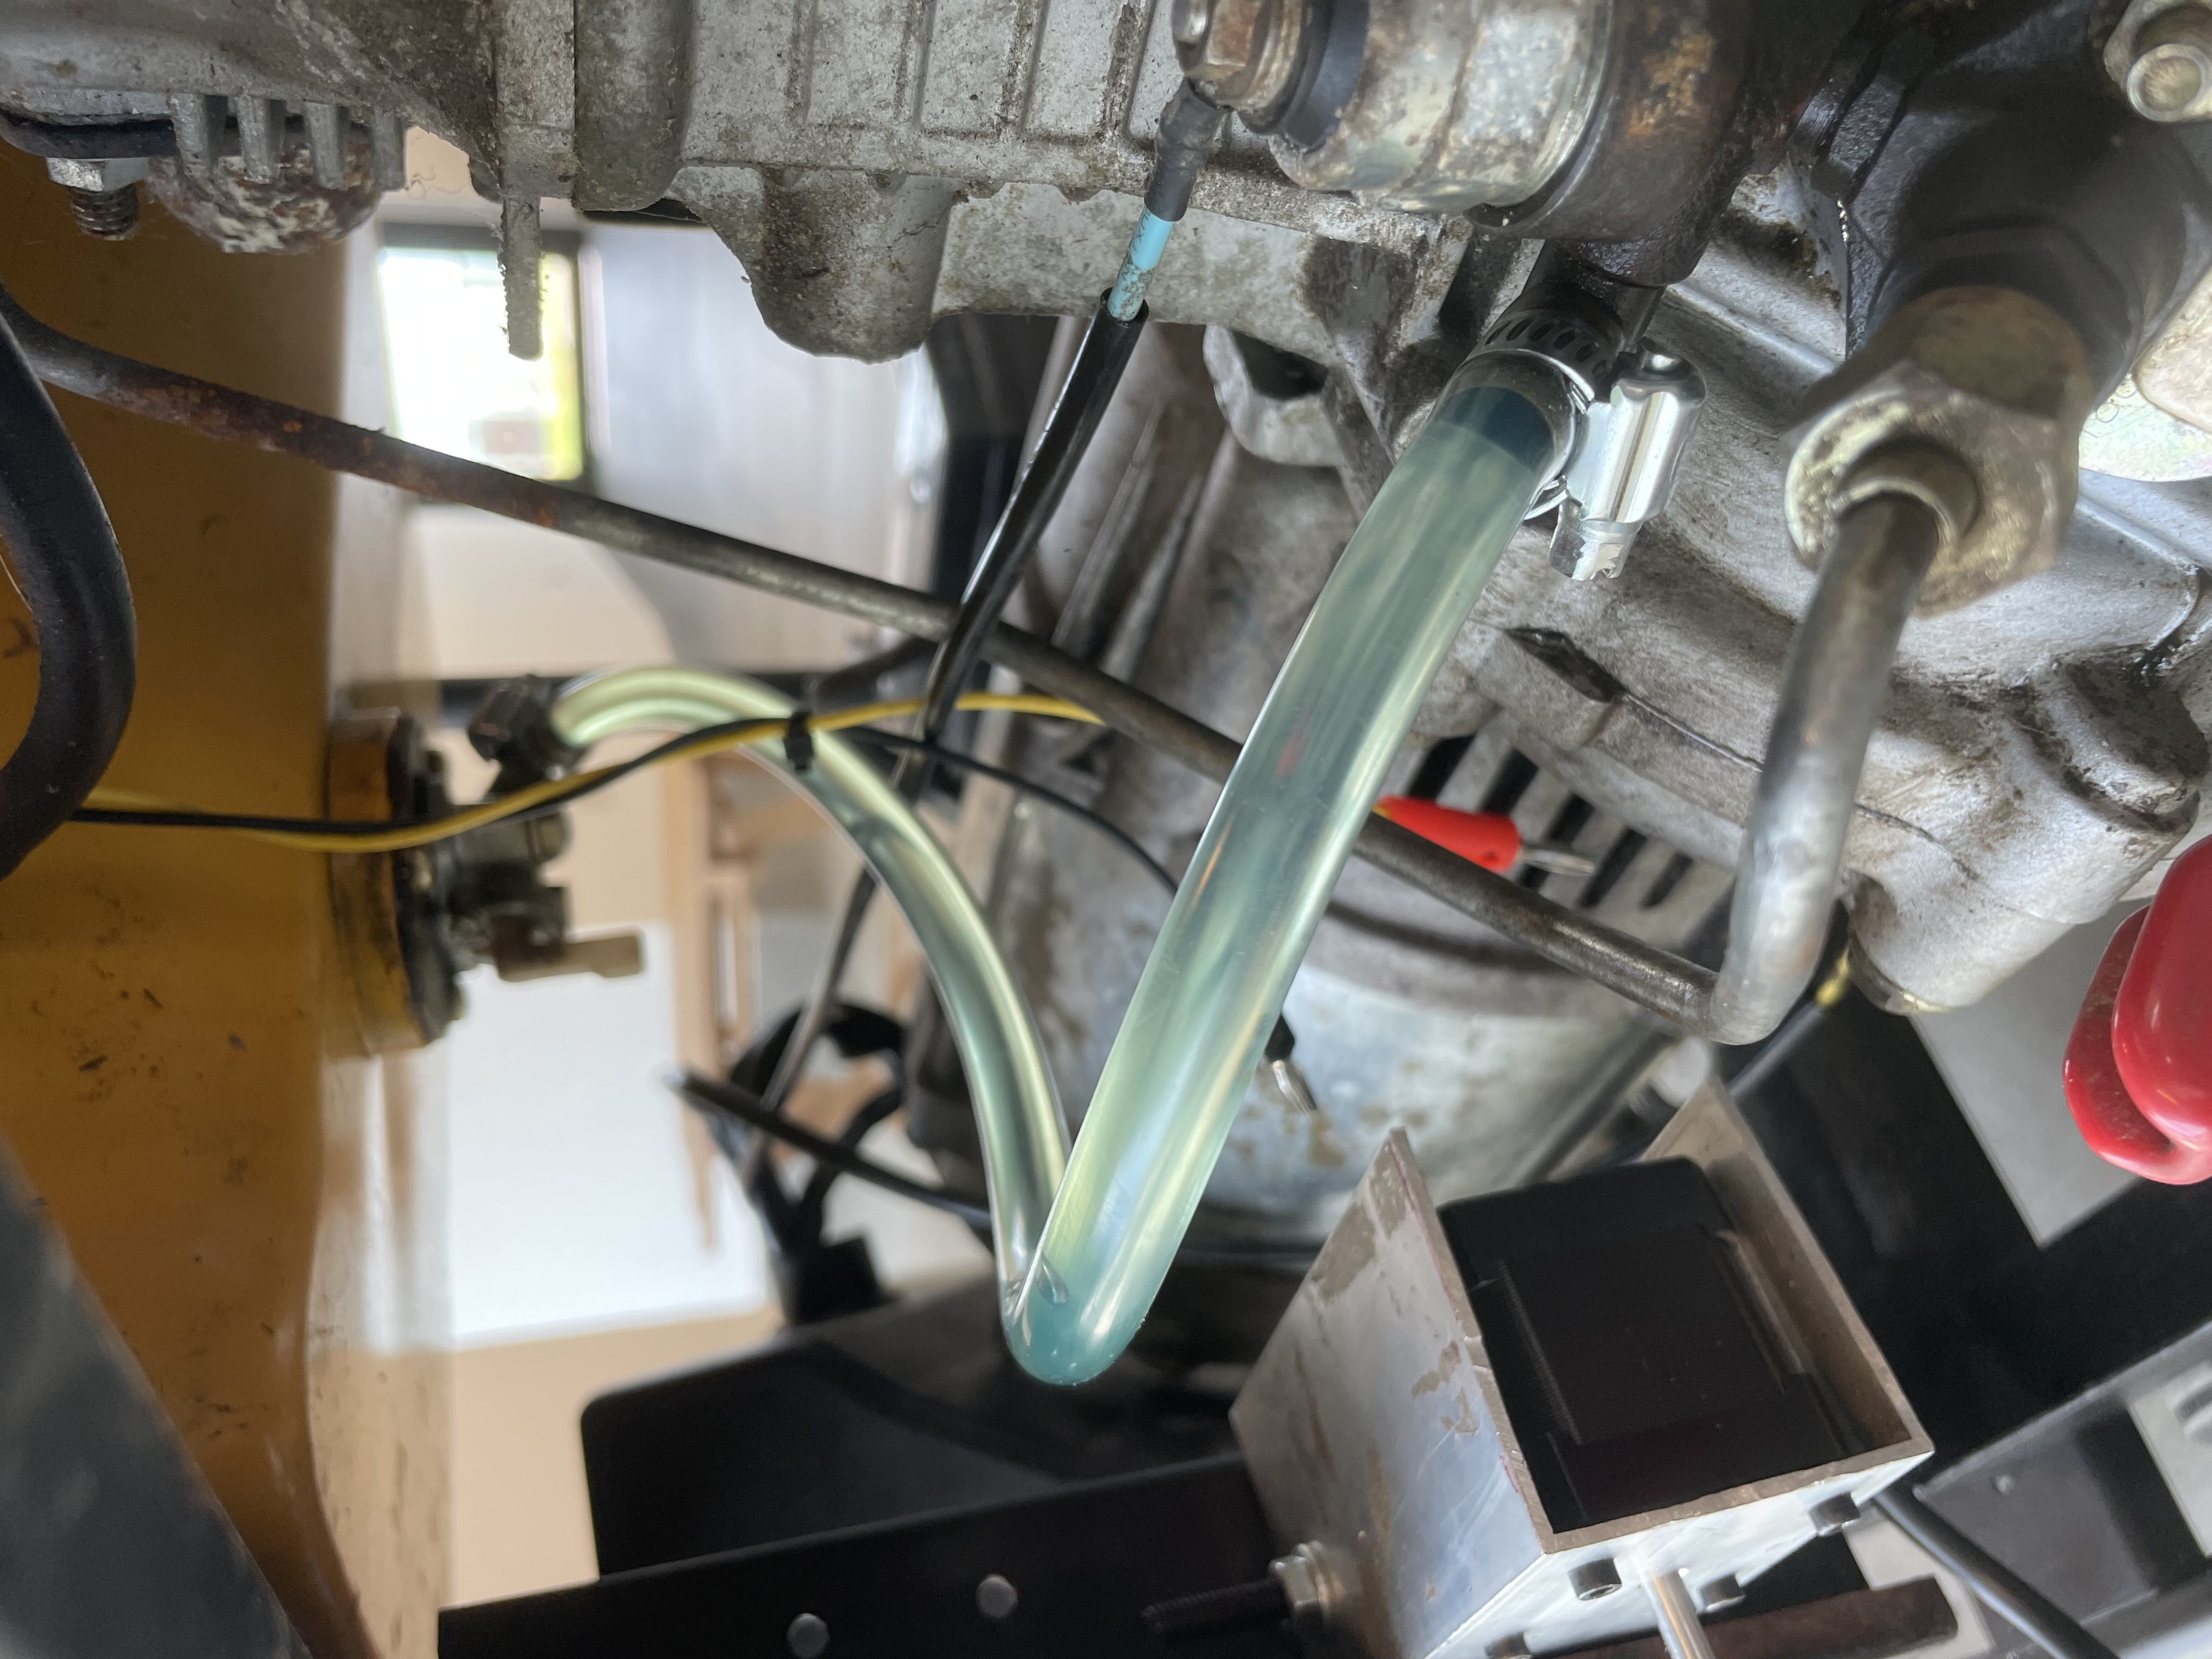
\includegraphics[angle = 270, width=0.75\linewidth]{IMG_4727.jpeg}
    \caption{Dodato crevo}
  \end{minipage}
\end{figure}


Nakon toga je usledilo istraživanje kako je povezana kontrolna tabla sa samim motorom i crtanje šeme prema onome što vidimo, da bismo mogli da zaključimo gde možemo povezati naš Arduino koji će pokretati celu logiku. Paralelno sa crtanjem šeme je proveravana struja solenoida. \\

\begin{figure}[htbp]
  \centering
  \begin{minipage}[b]{0.3\textwidth}
    \centering
    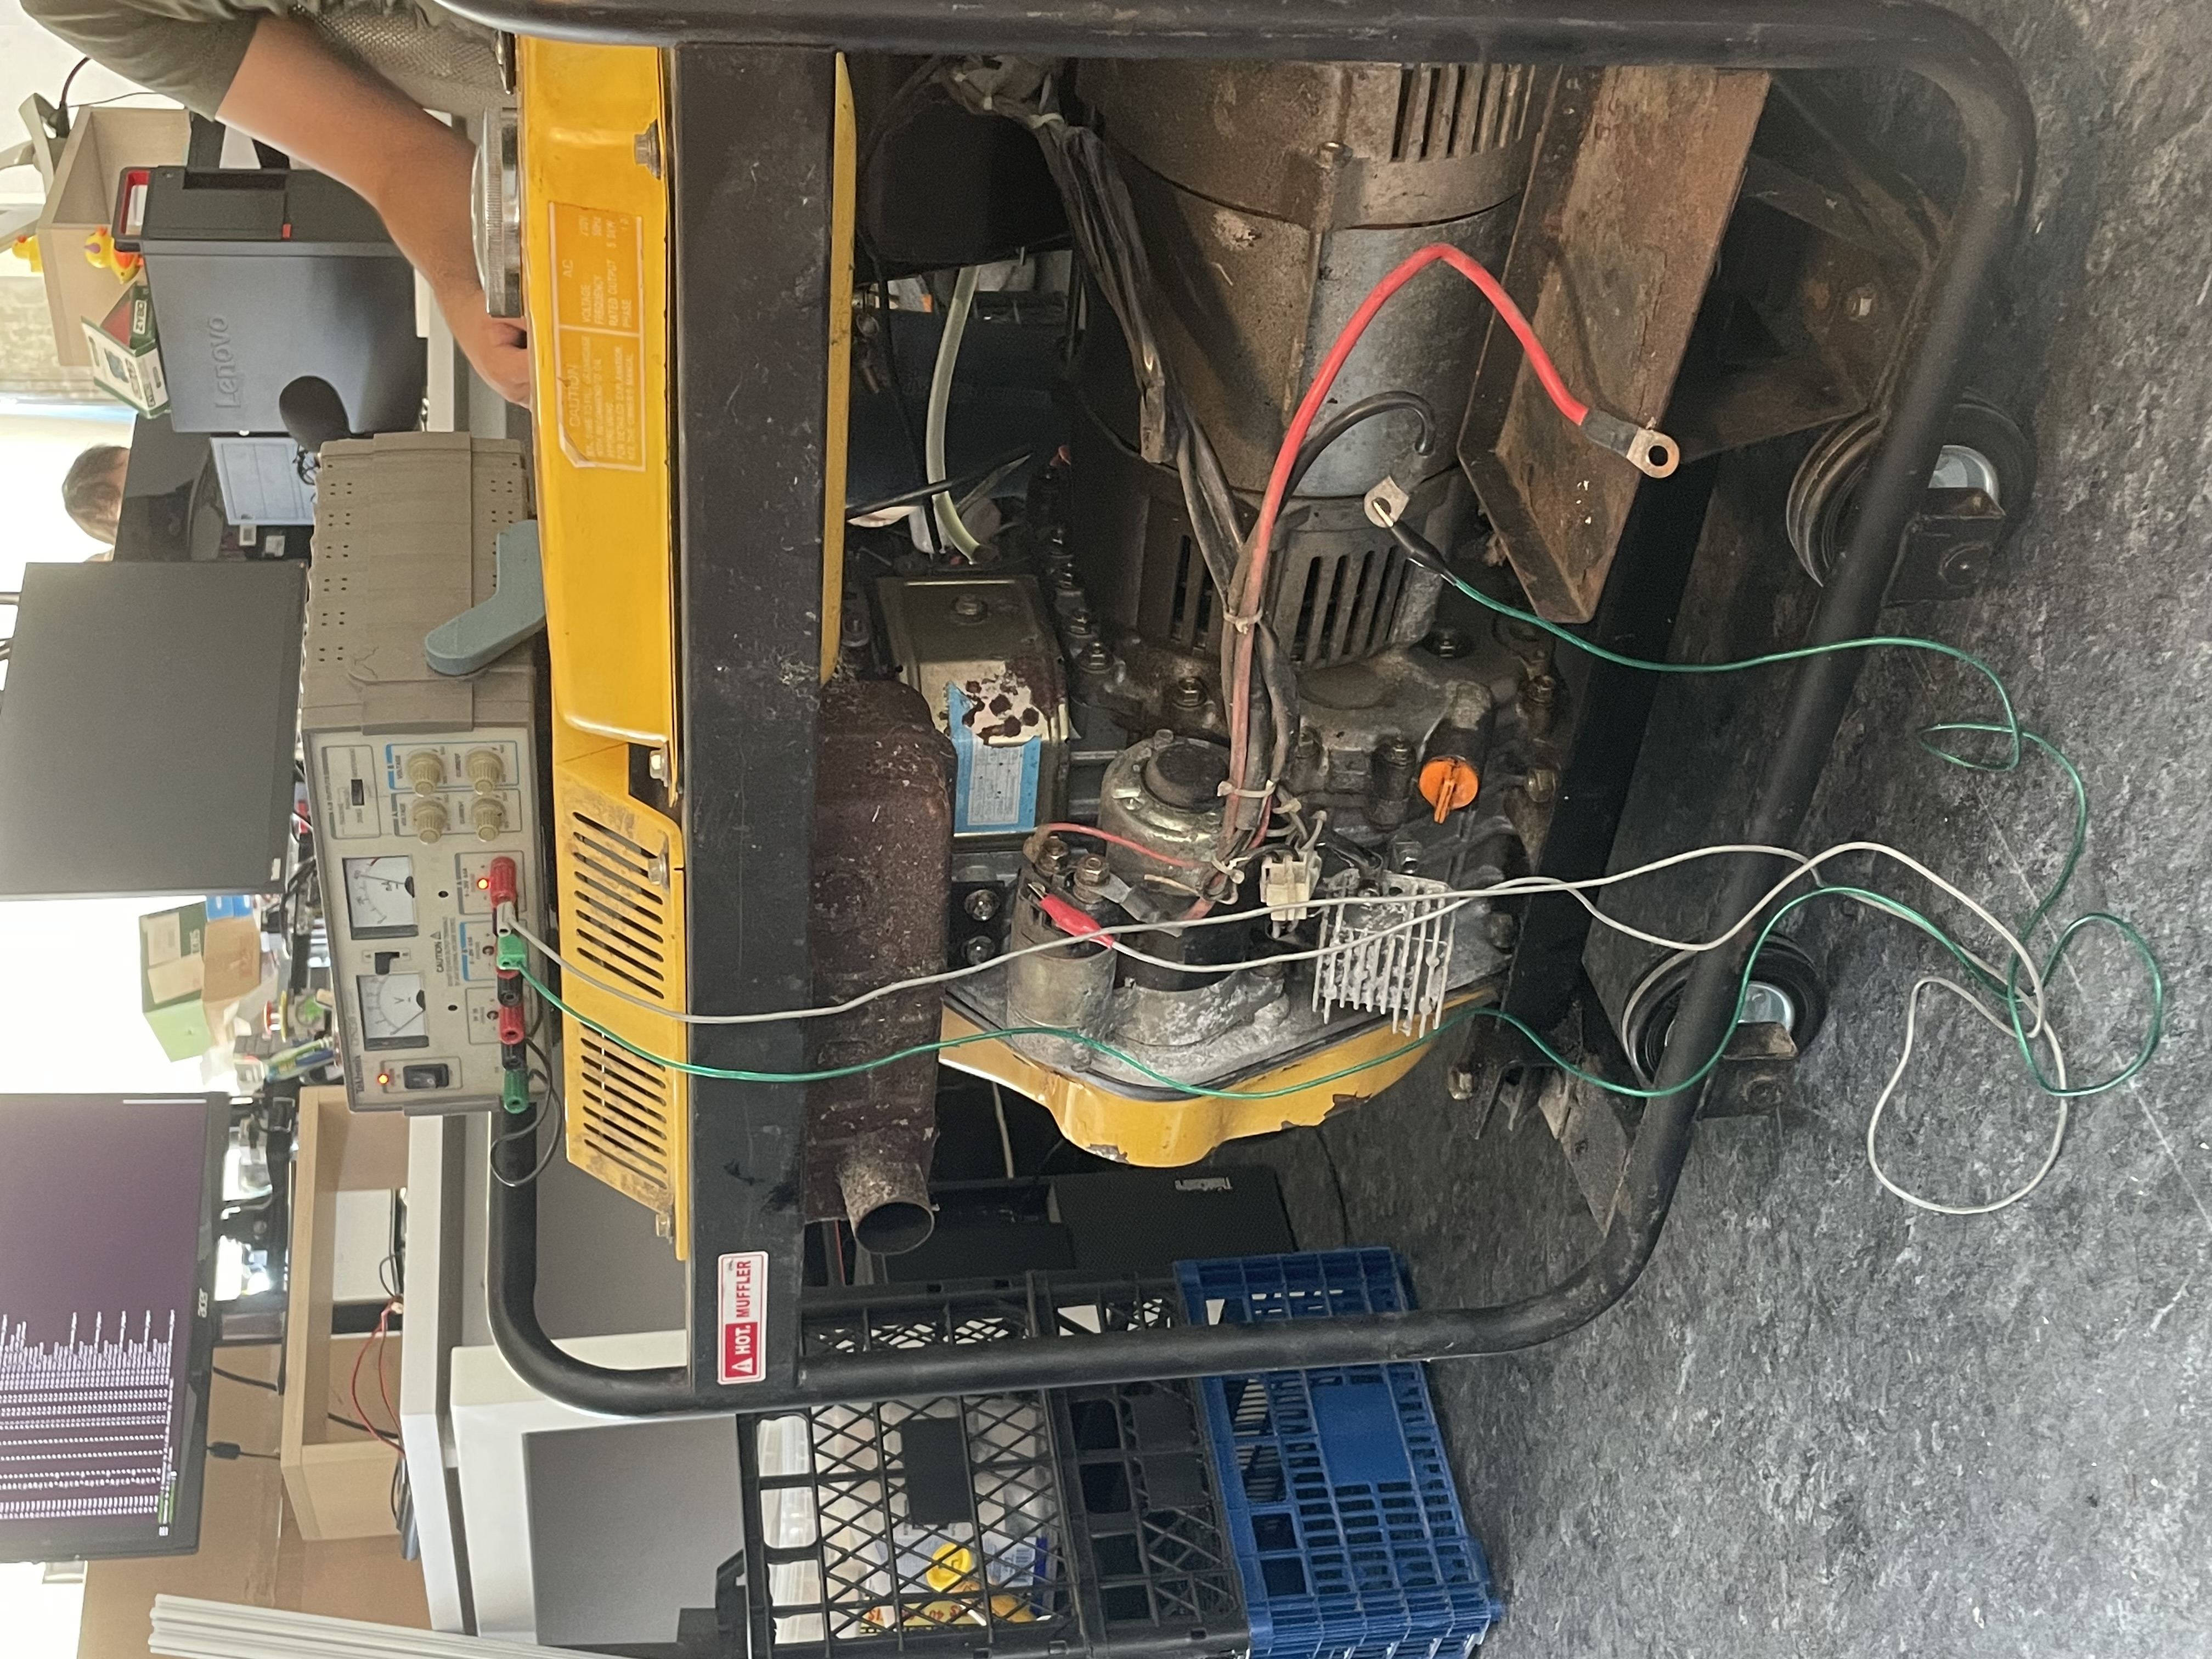
\includegraphics[angle = 270, width=0.75\linewidth]{IMG_4331.jpeg}
    \caption{Merenje solenoida}
  \end{minipage}
  \hfill
  \begin{minipage}[b]{0.3\textwidth}
    \centering
    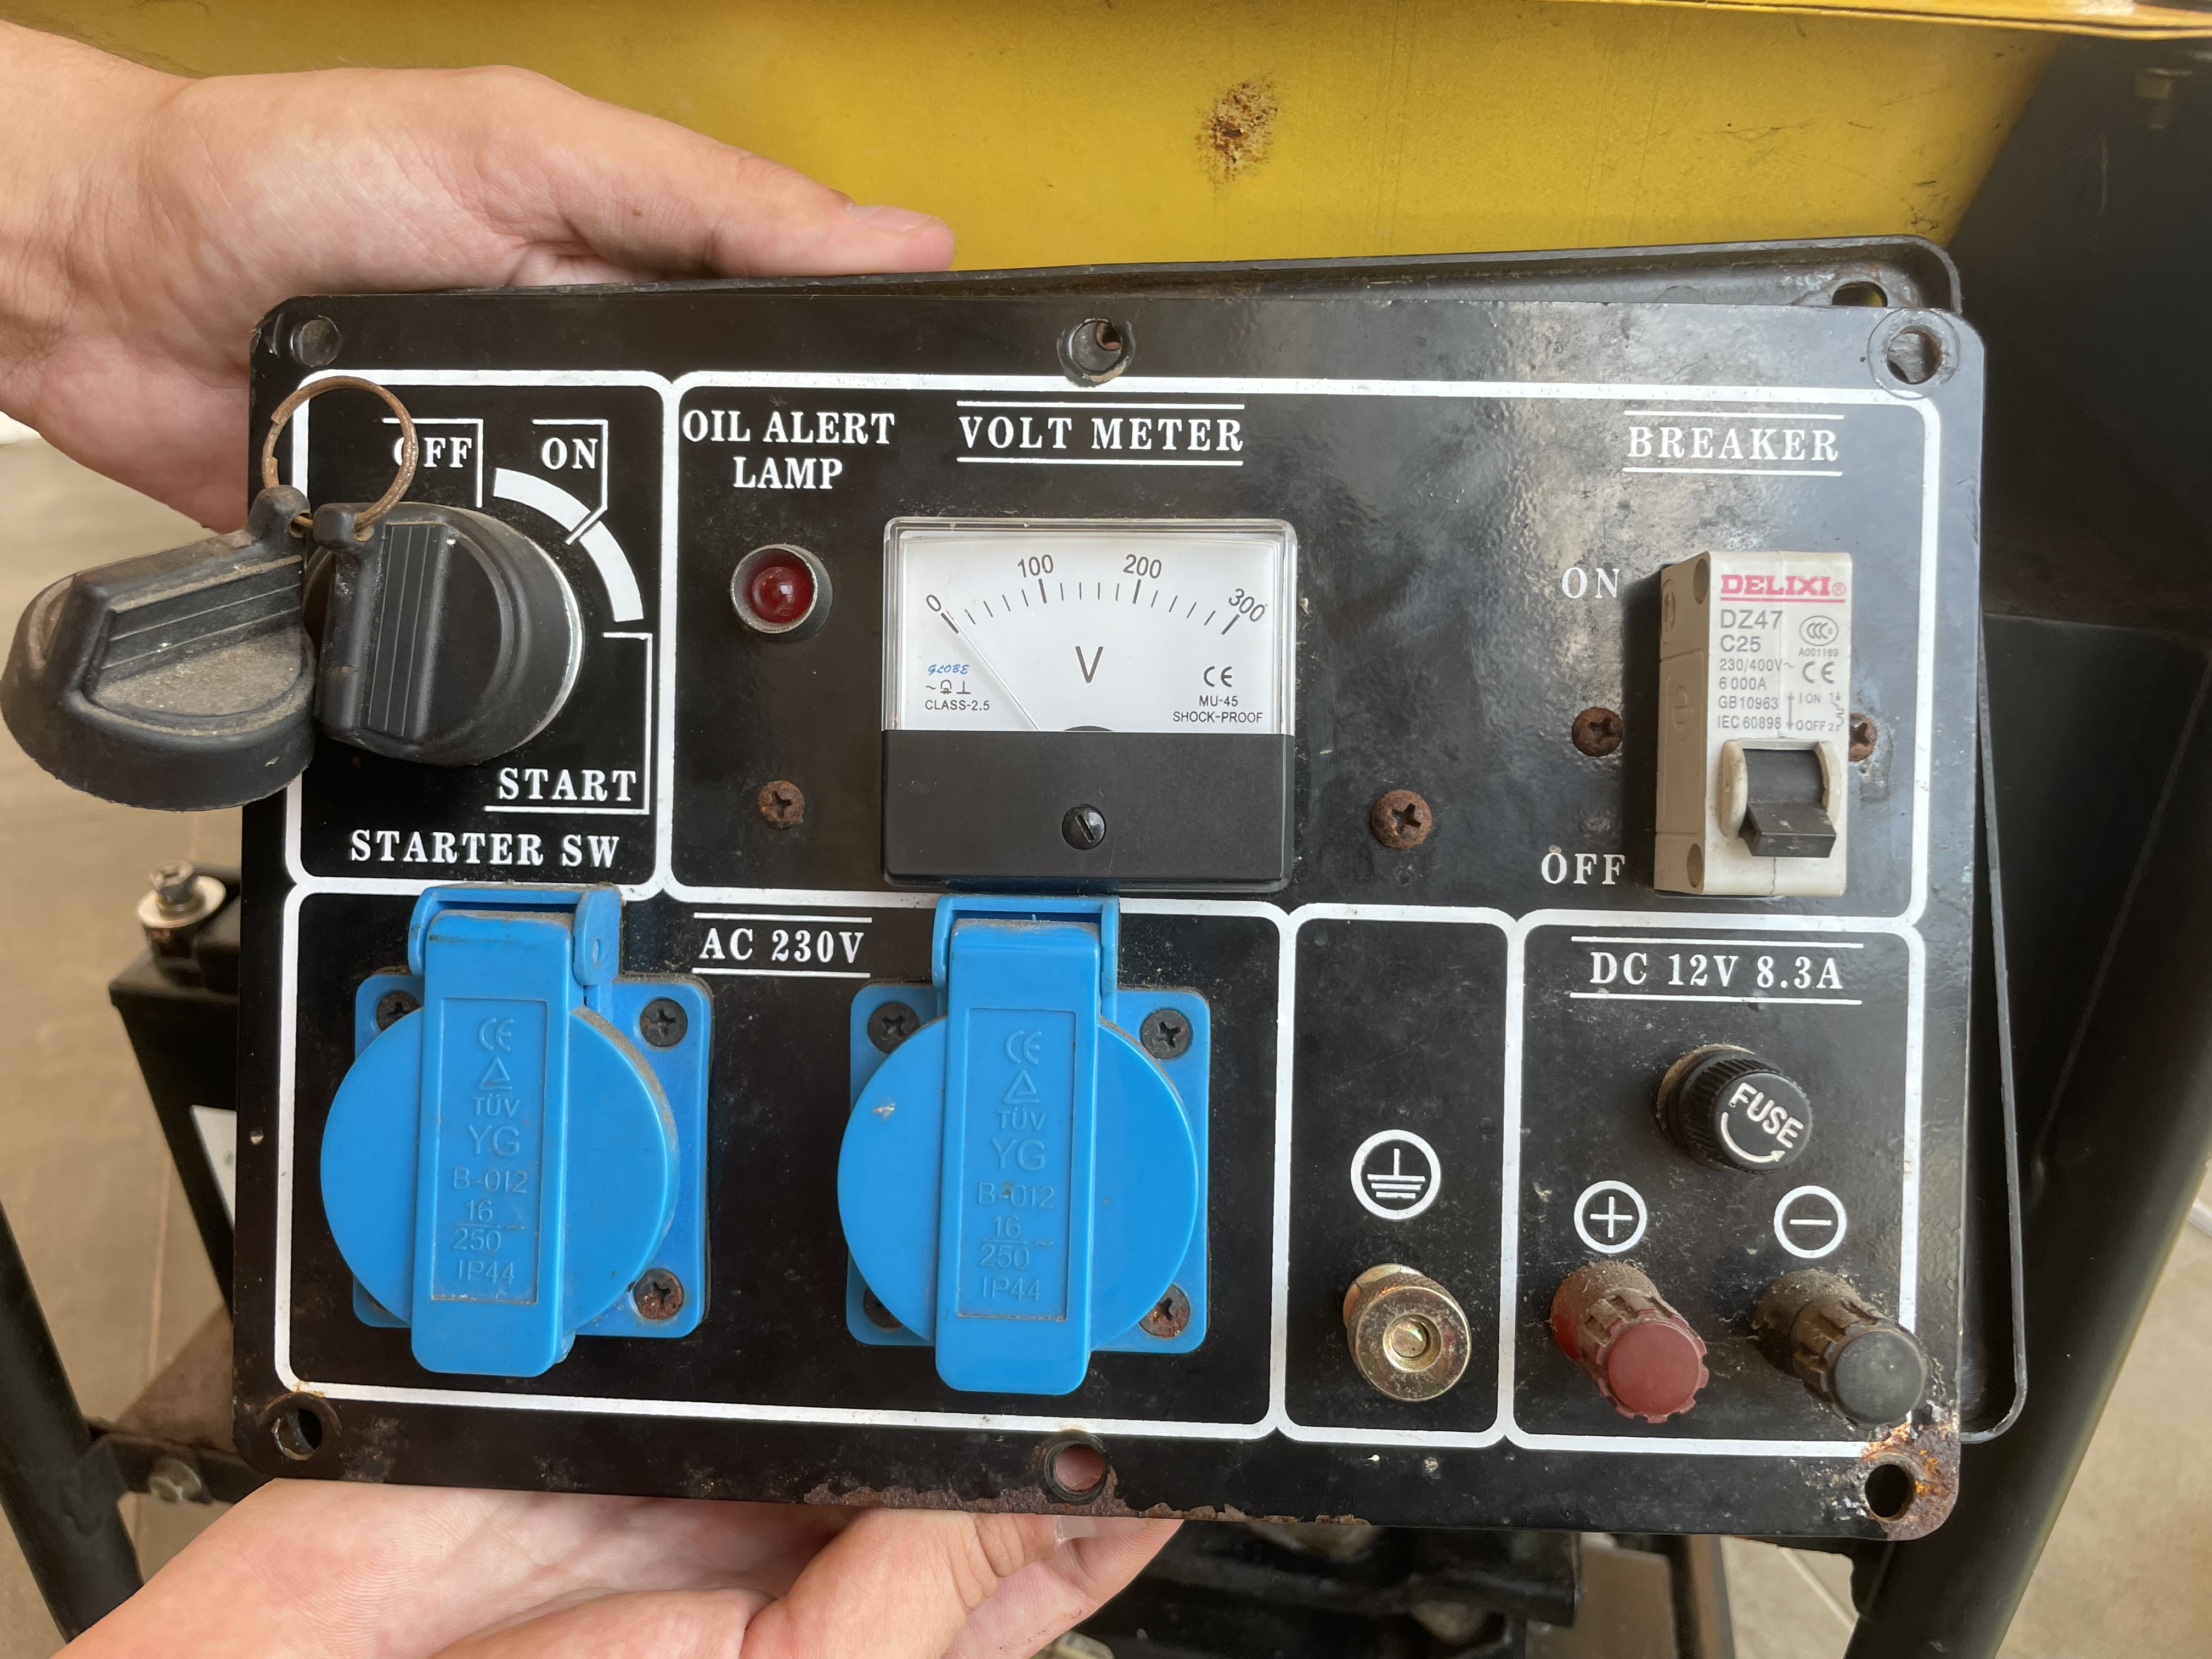
\includegraphics[ width=0.75\linewidth]{IMG_4724.jpeg}
    \caption{Kontrolna tabla}
  \end{minipage}
    \hfill
  \begin{minipage}[b]{0.3\textwidth}
    \centering
    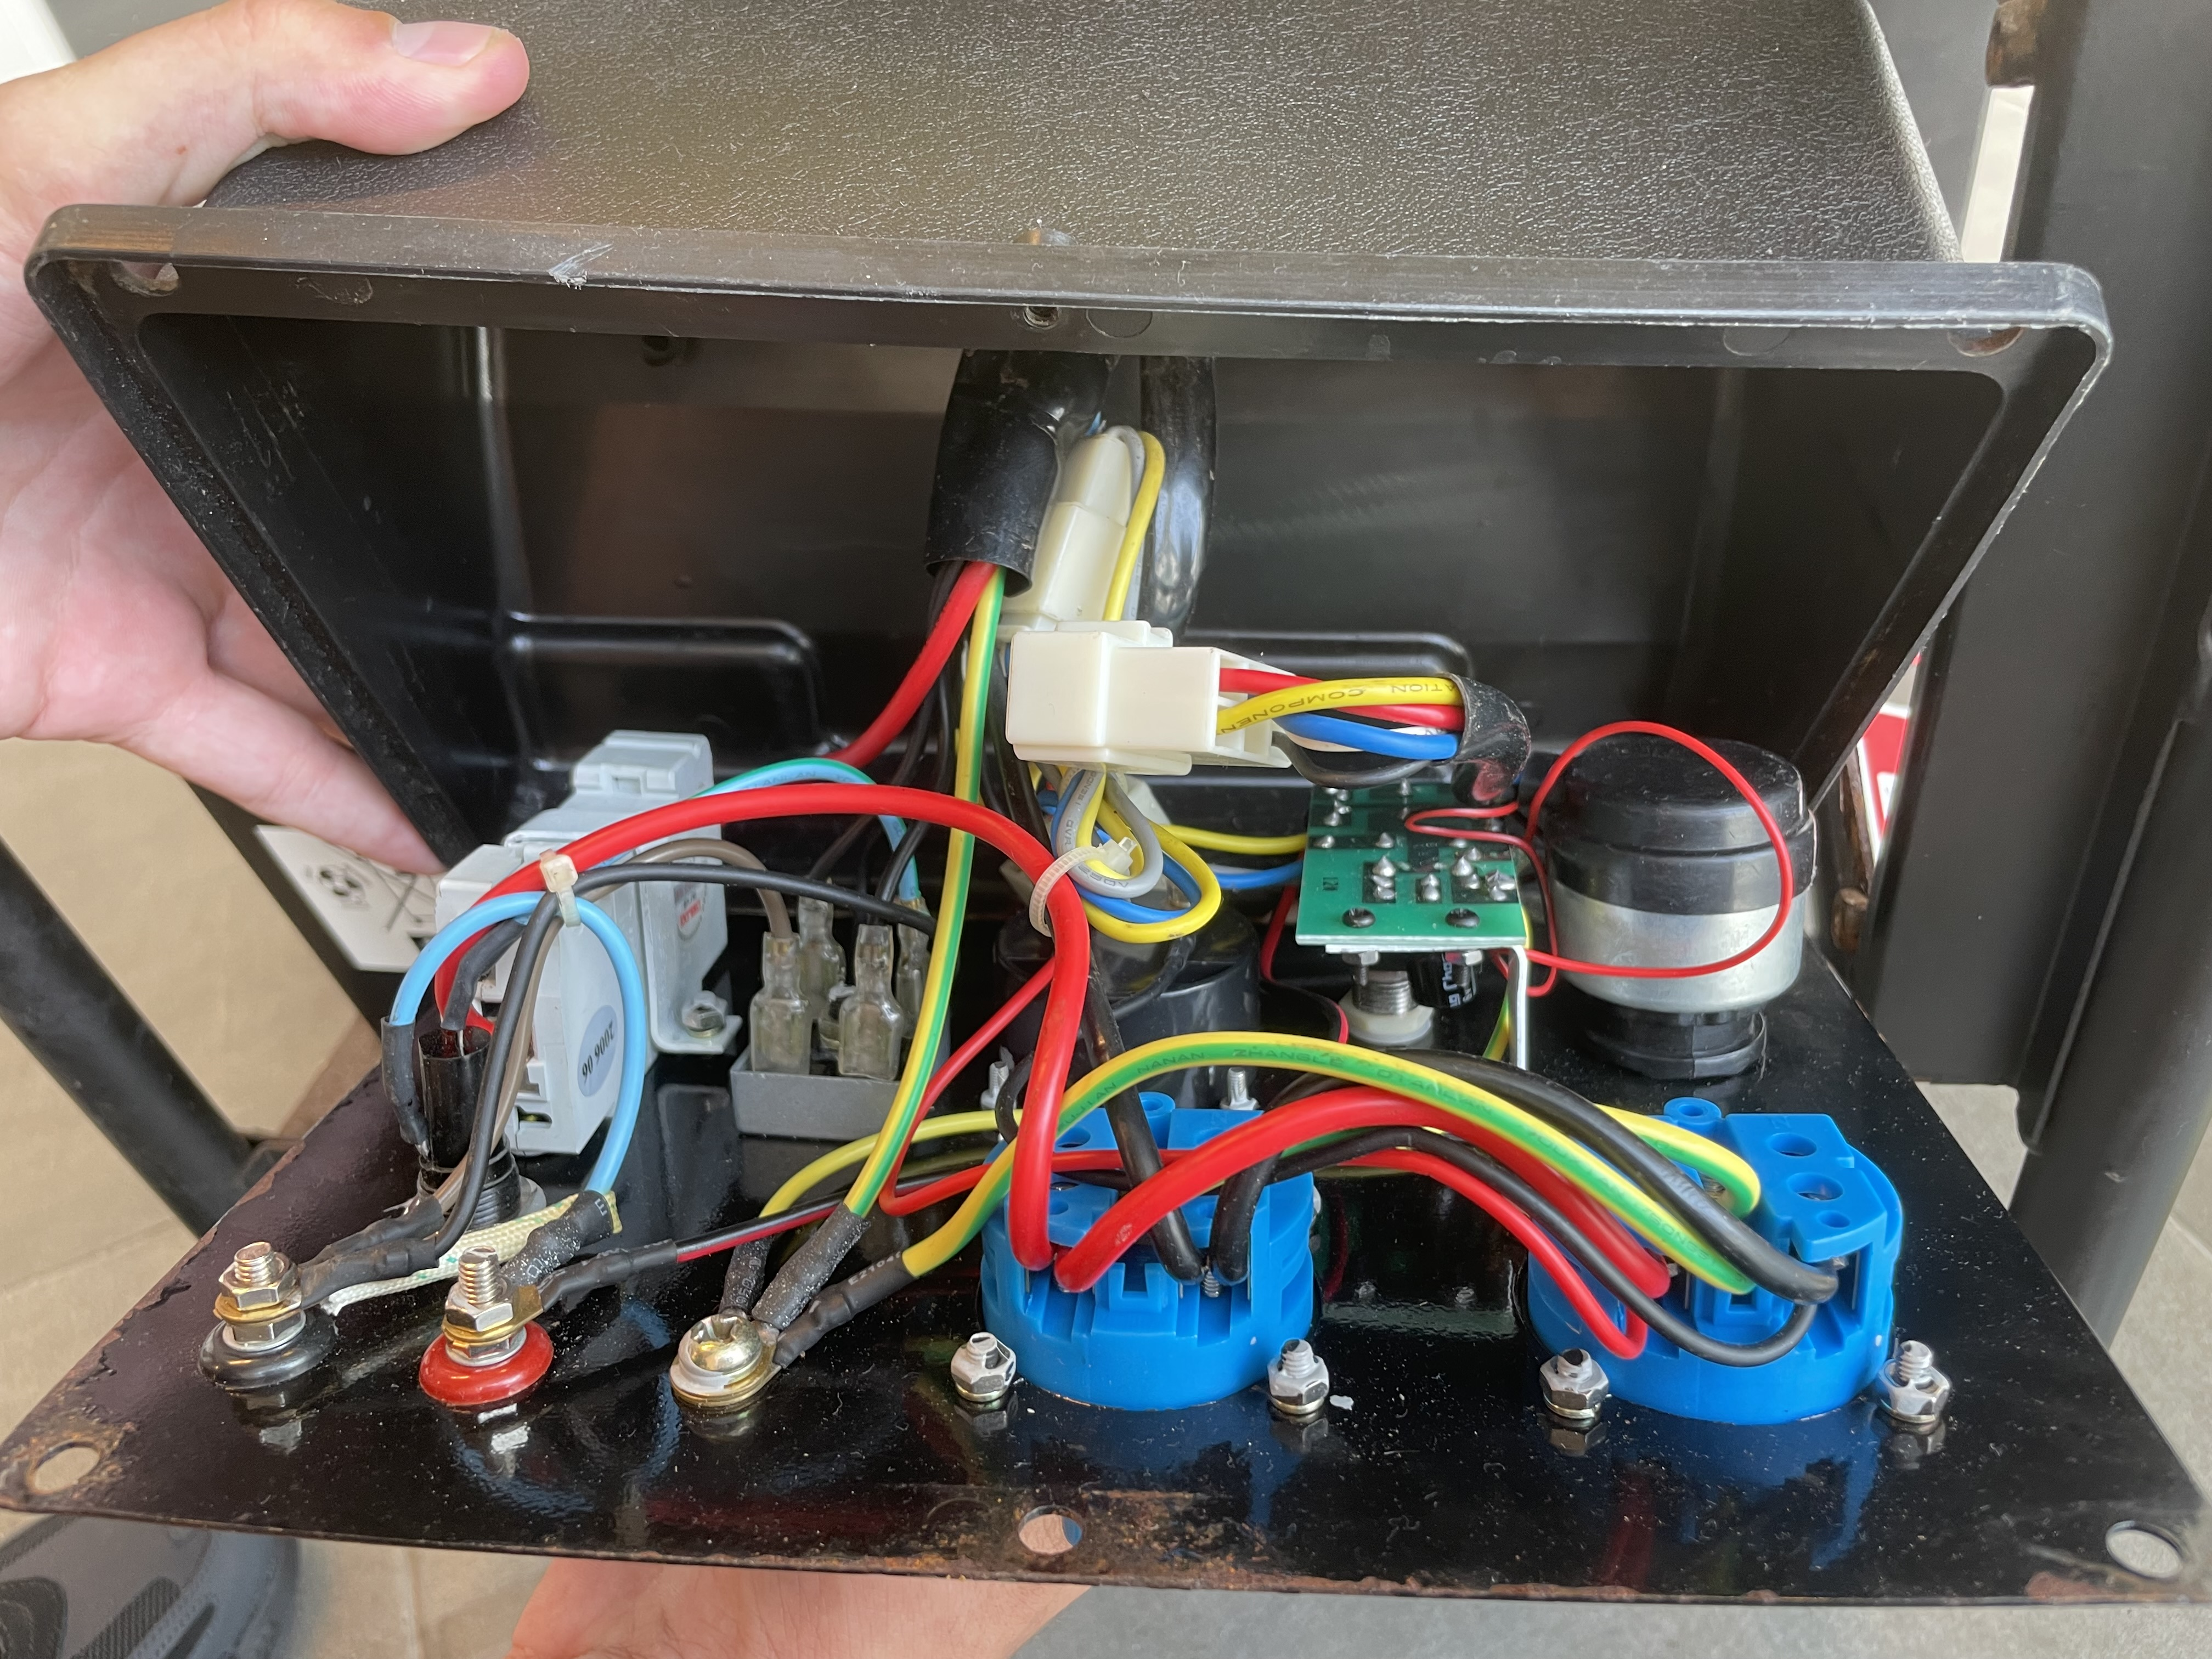
\includegraphics[ width=0.75\linewidth]{IMG_4722.jpeg}
    \caption{Iza kontrolne table}
  \end{minipage}
\end{figure}


Nakon nacrtane cele šeme motora i kontrolne table, usledilo je montiranje step motora na mašinu i pisanje rutine za njega, koji će da pokreće menjač. \\ 

\begin{figure}[htbp]
  \begin{minipage}[b]{0.3\textwidth}
    \centering
    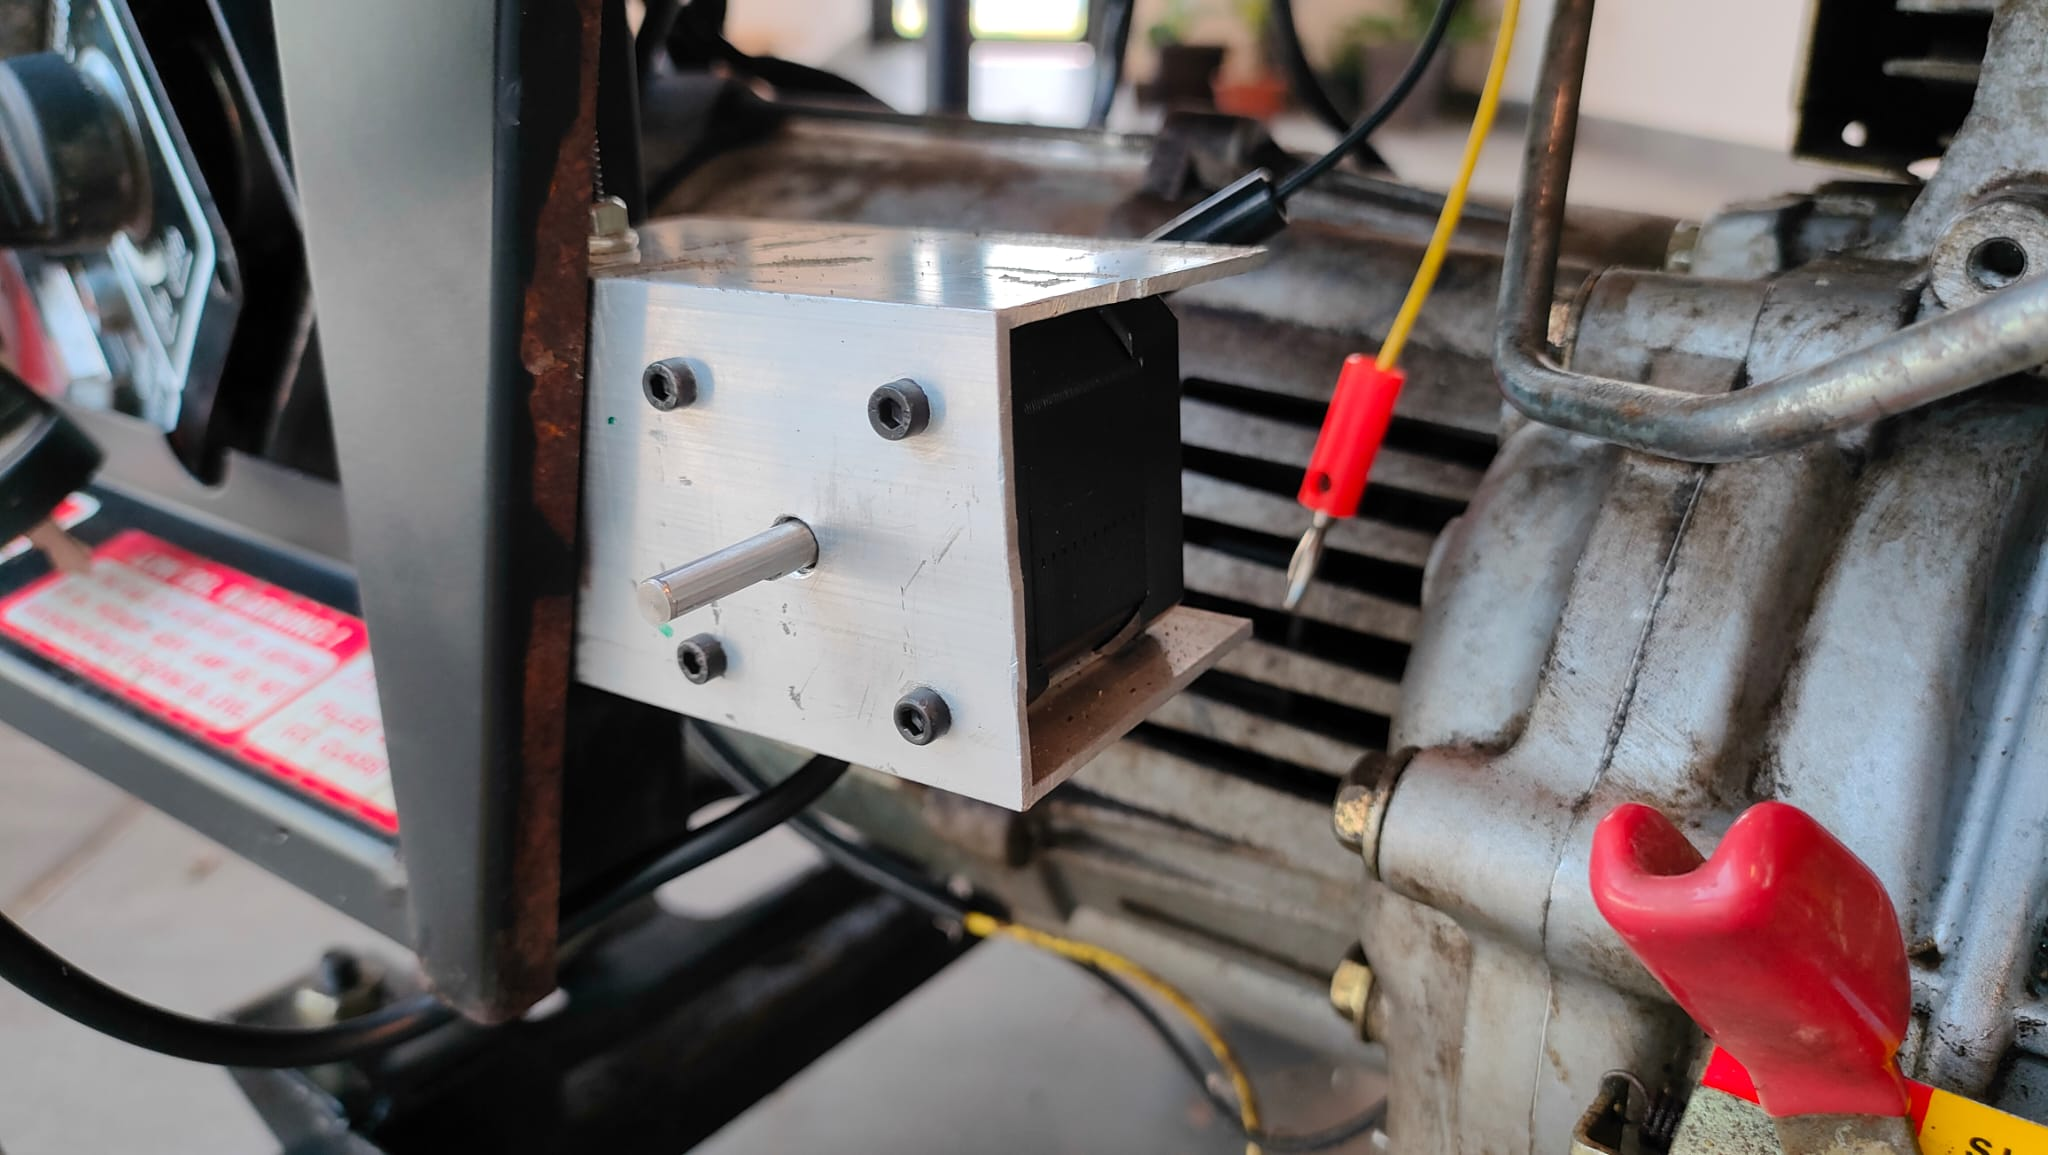
\includegraphics[ width=0.75\linewidth]{step.jpeg}
    \caption{Prva verzija step motora}
  \end{minipage}
\end{figure}

\newpage


Dalje, napravljene su dve pločice za arduino, jedna koja povezuje arduino sa samim motorom i vuče struju iz solenoida, a druga koja na sebi ima dugme za paljenje i potenciometar kojim možemo upravljati menjač, što je u suštini jedan od najbitnijih koraka ovog projekta. 
Kada je sve povezano, napisan je kod za pokretanje dugmeta i za potencimetar i spajanje sa step motorom, što je poslednji korak ovog projekta. 

\begin{figure}[htbp]
  \centering
  \begin{minipage}[b]{0.3\textwidth}
    \centering
    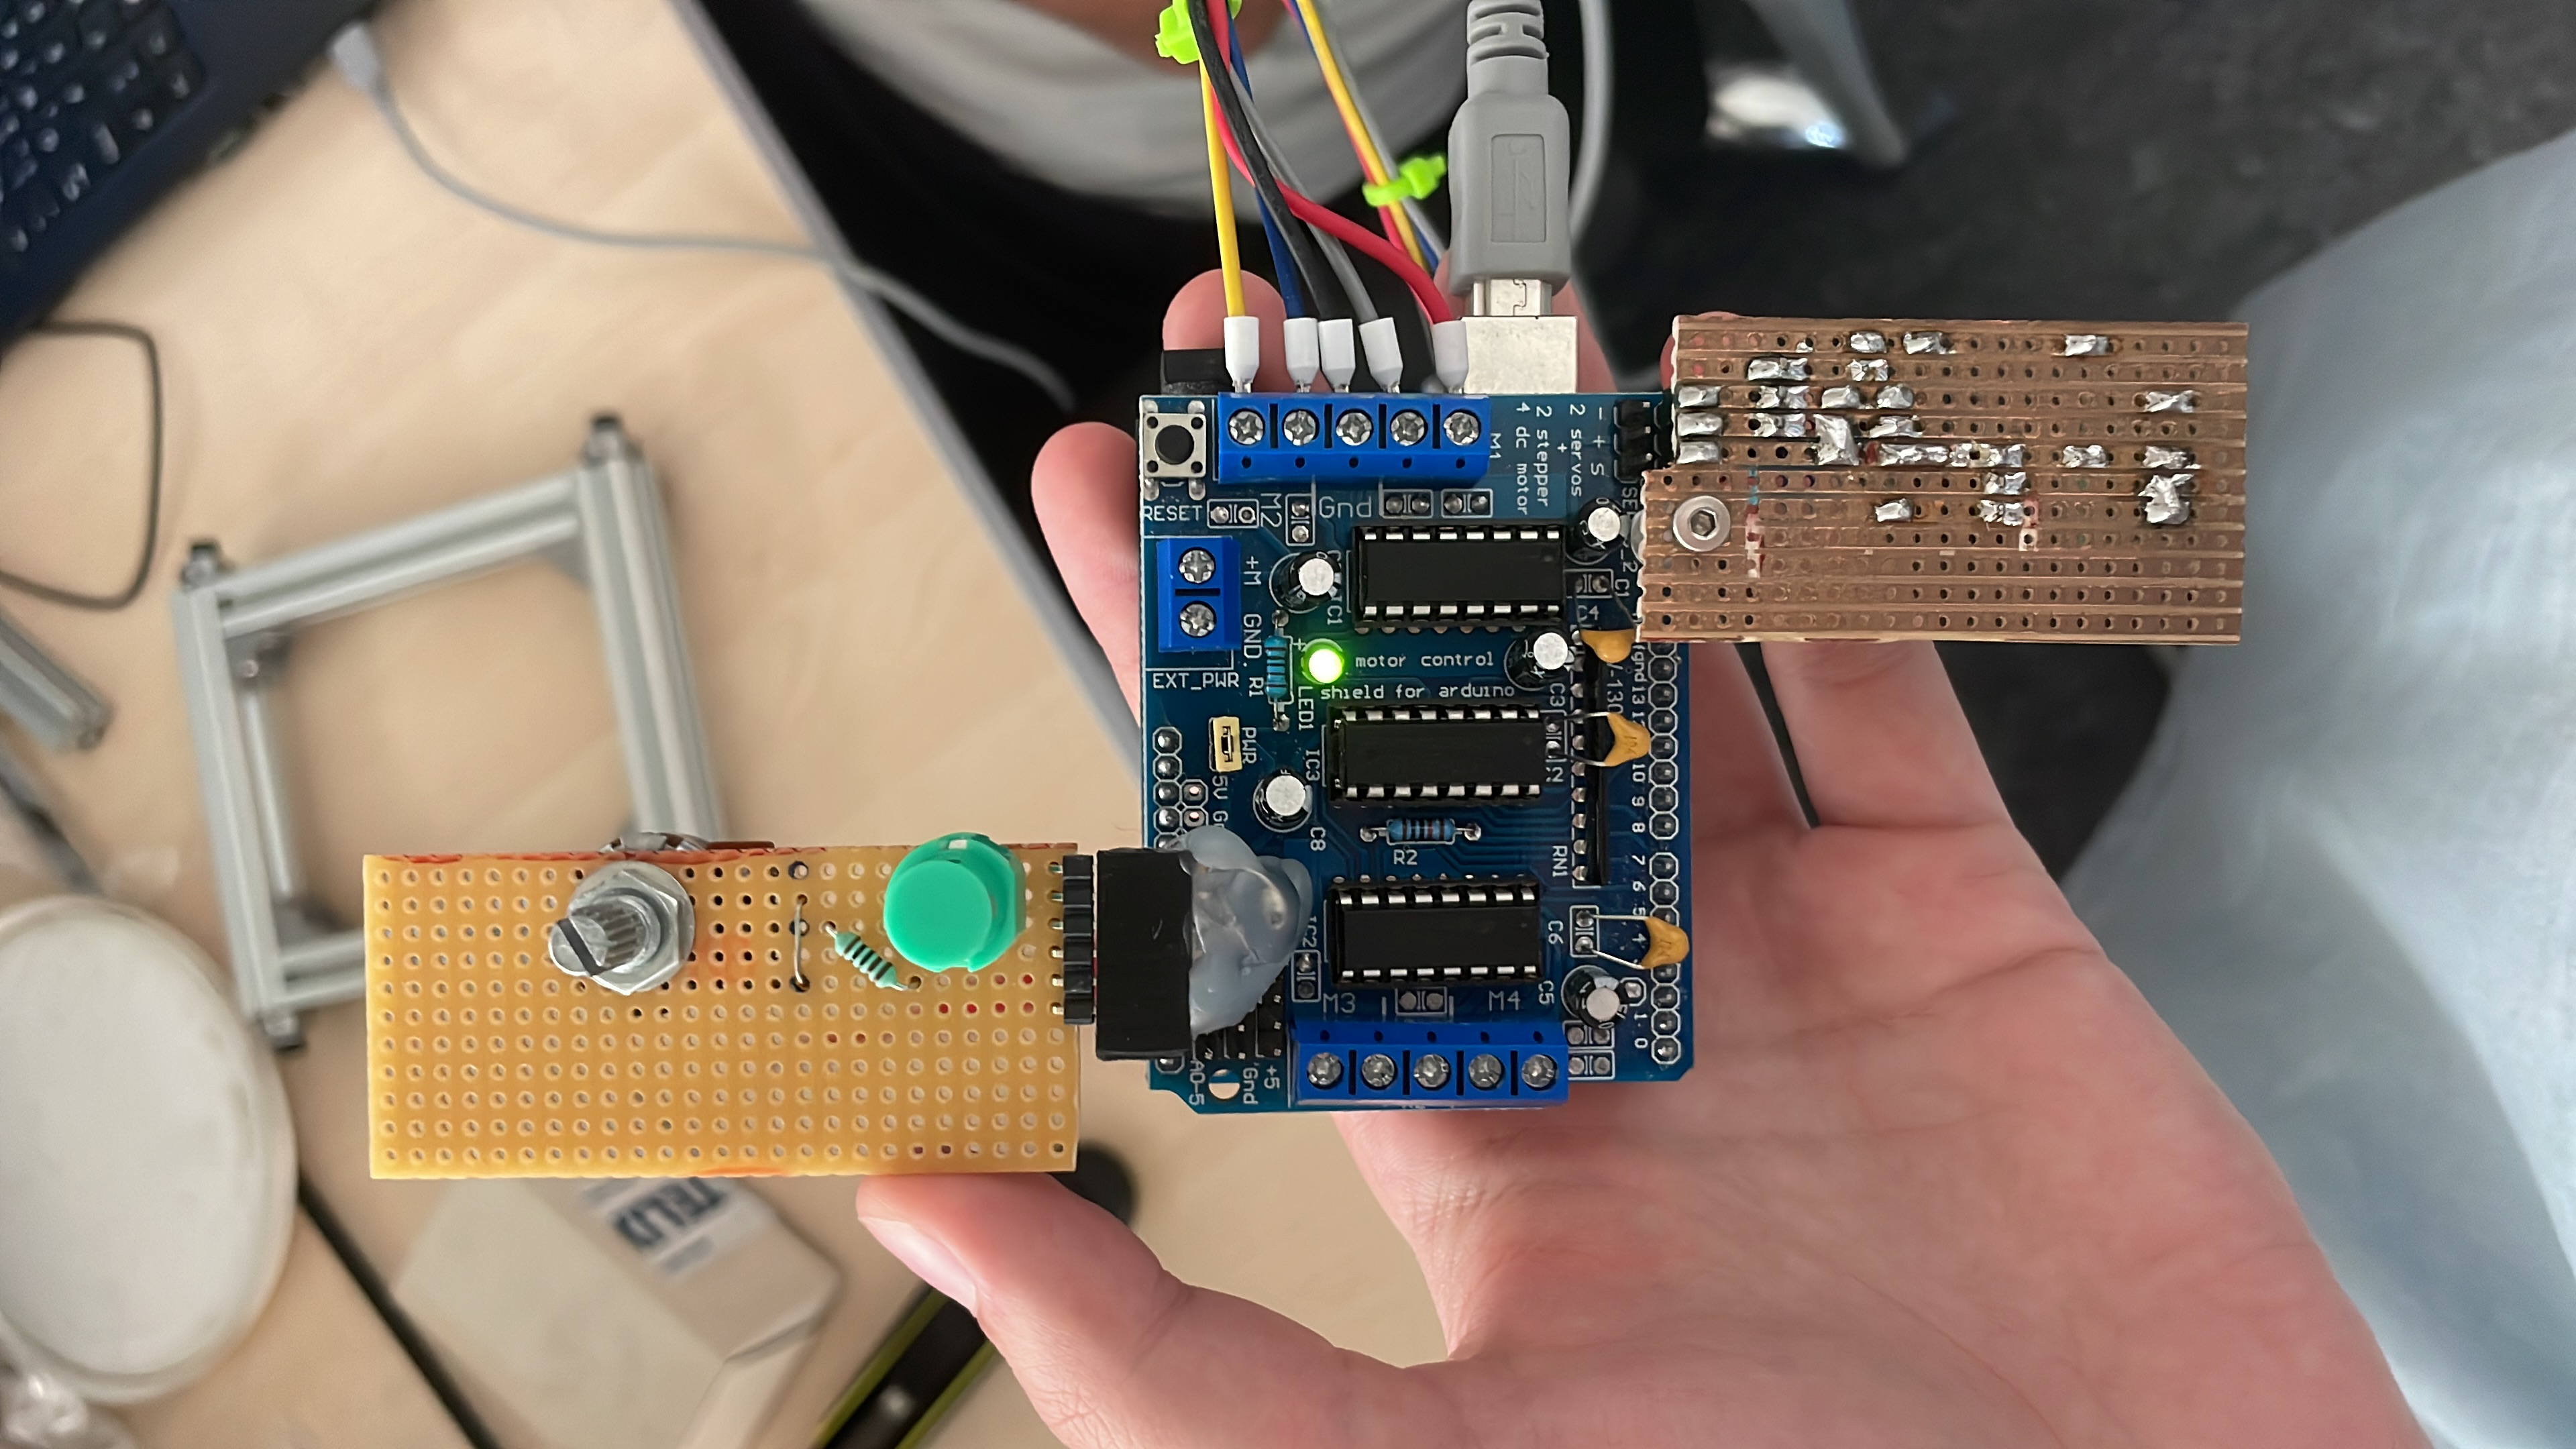
\includegraphics[angle = 270, width=0.75\linewidth]{frontside.jpeg}
    \caption{Plocica}
  \end{minipage}
  \hfill
  \begin{minipage}[b]{0.3\textwidth}
    \centering
    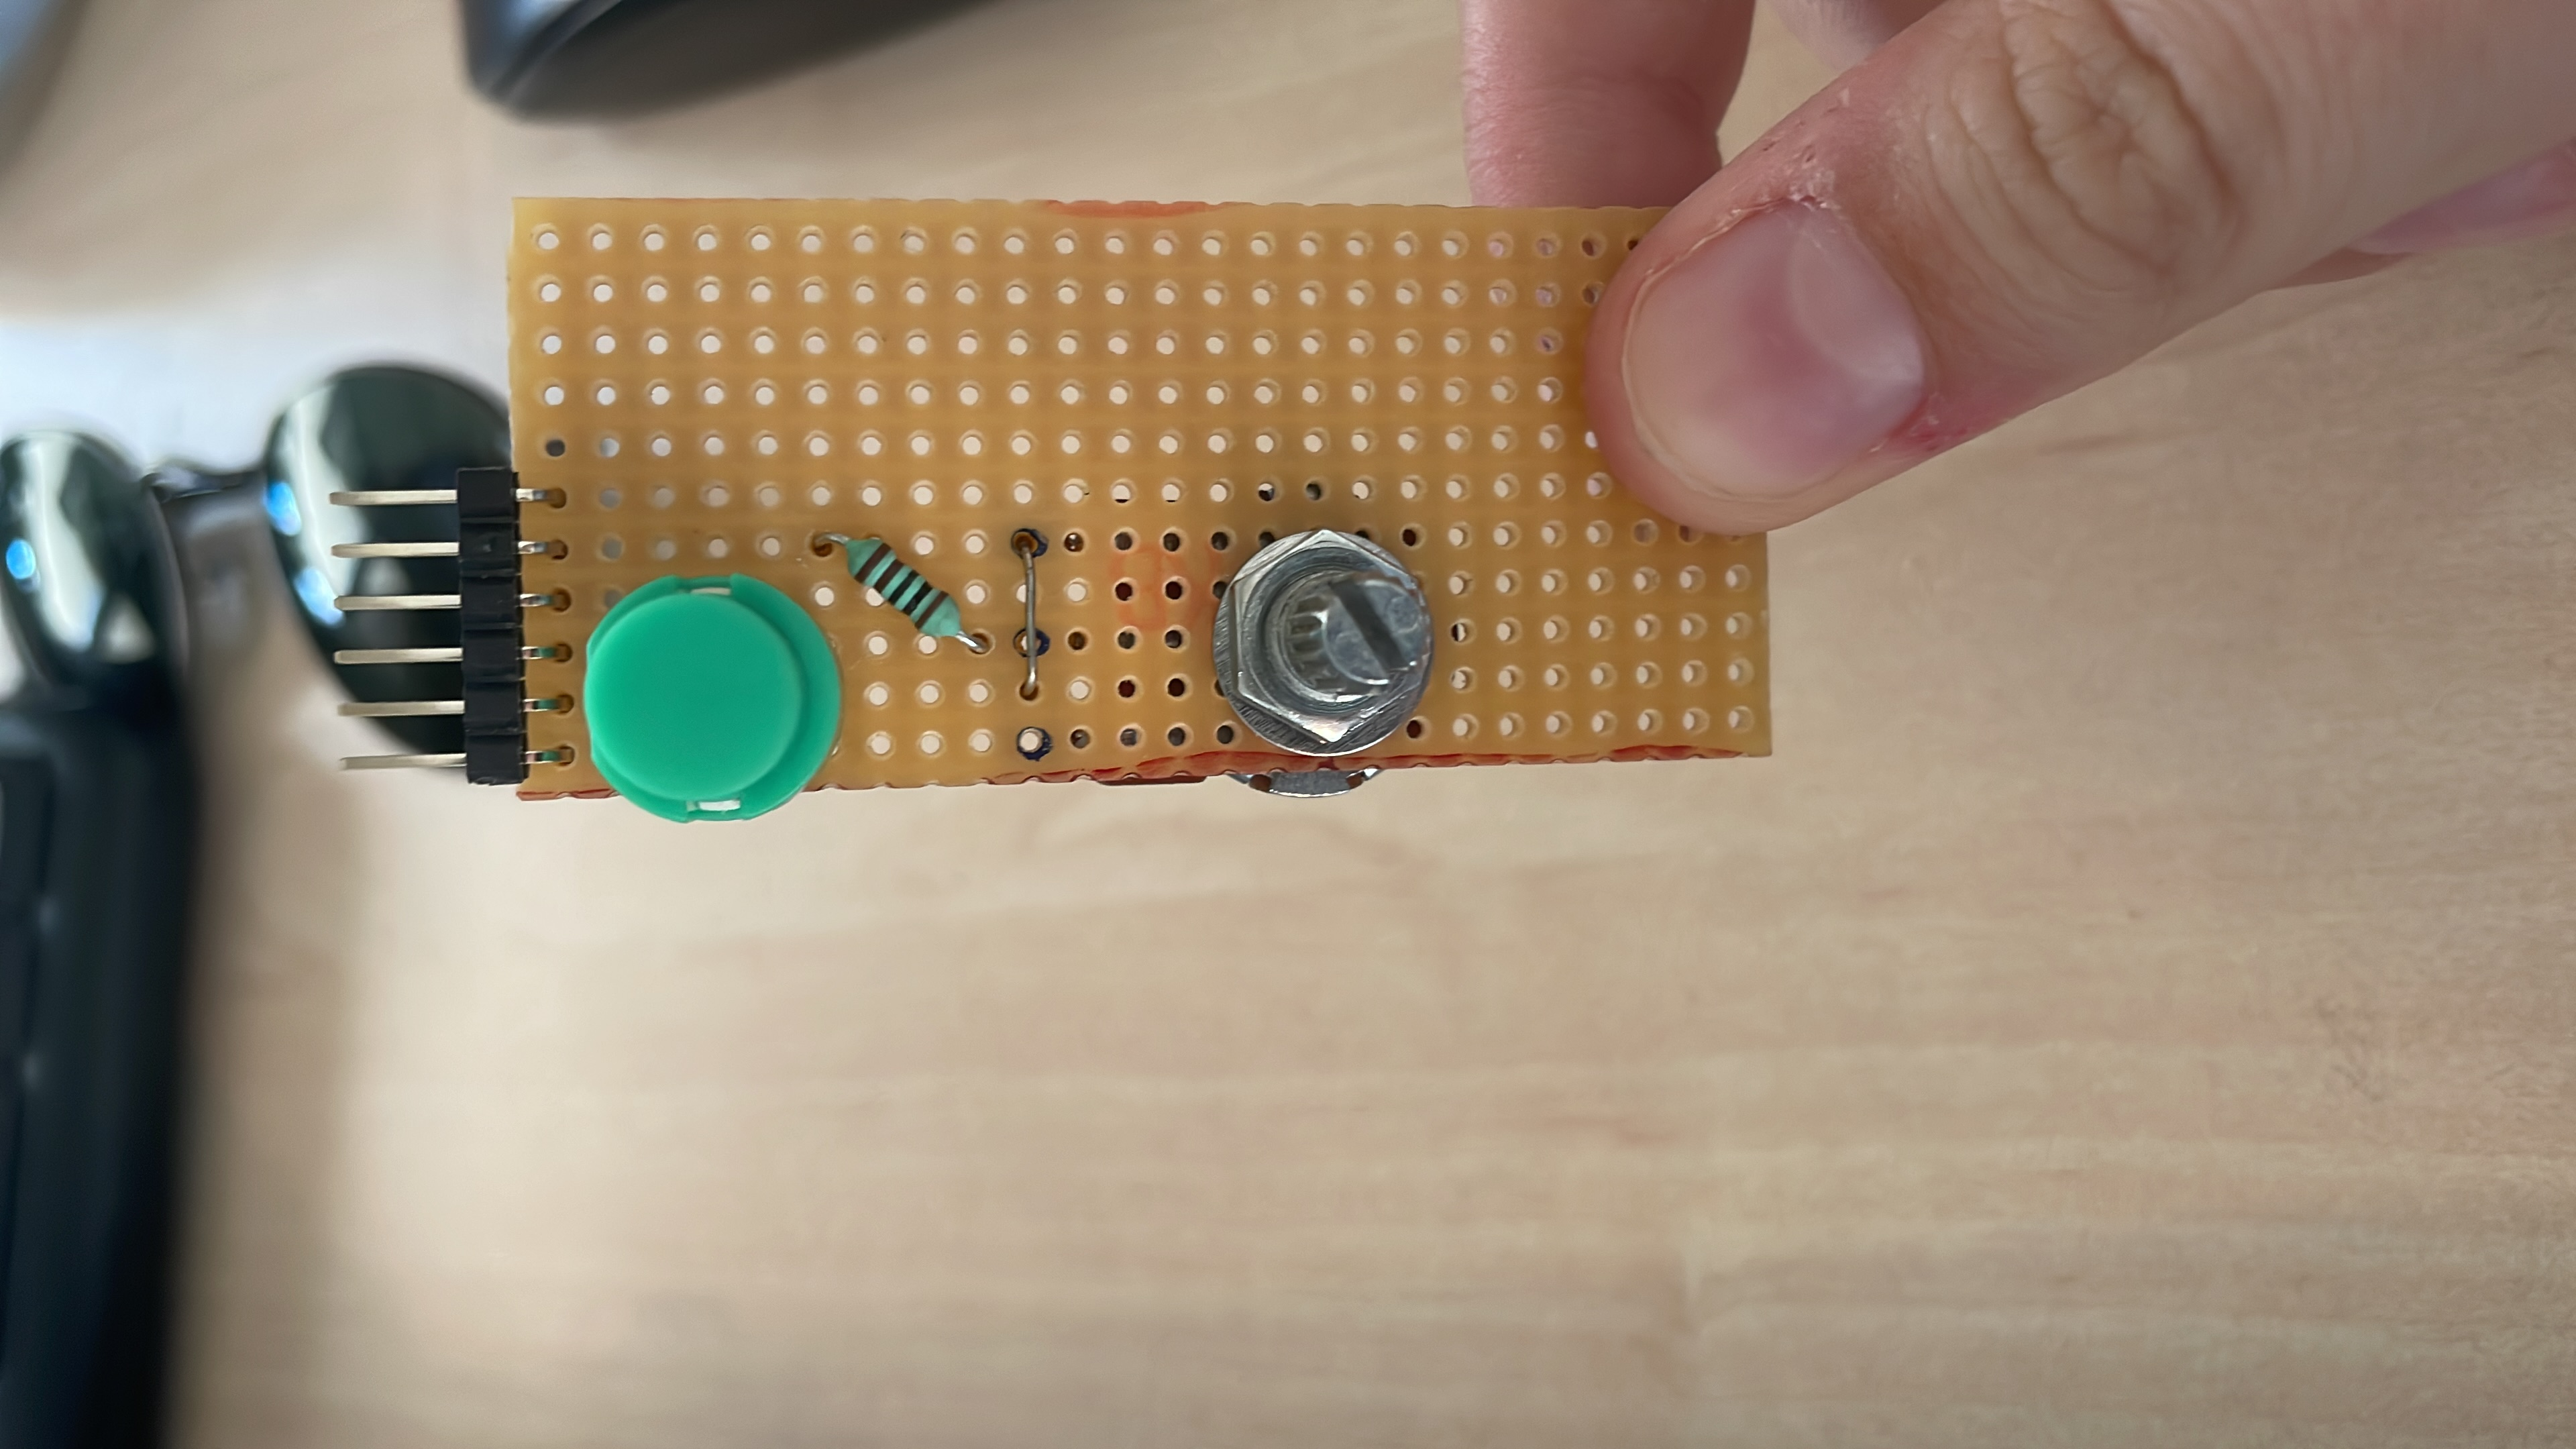
\includegraphics[ angle = 270,width=0.75\linewidth]{plocica.jpeg}
    \caption{tabla}
  \end{minipage}
    \hfill
  \begin{minipage}[b]{0.3\textwidth}
    \centering
    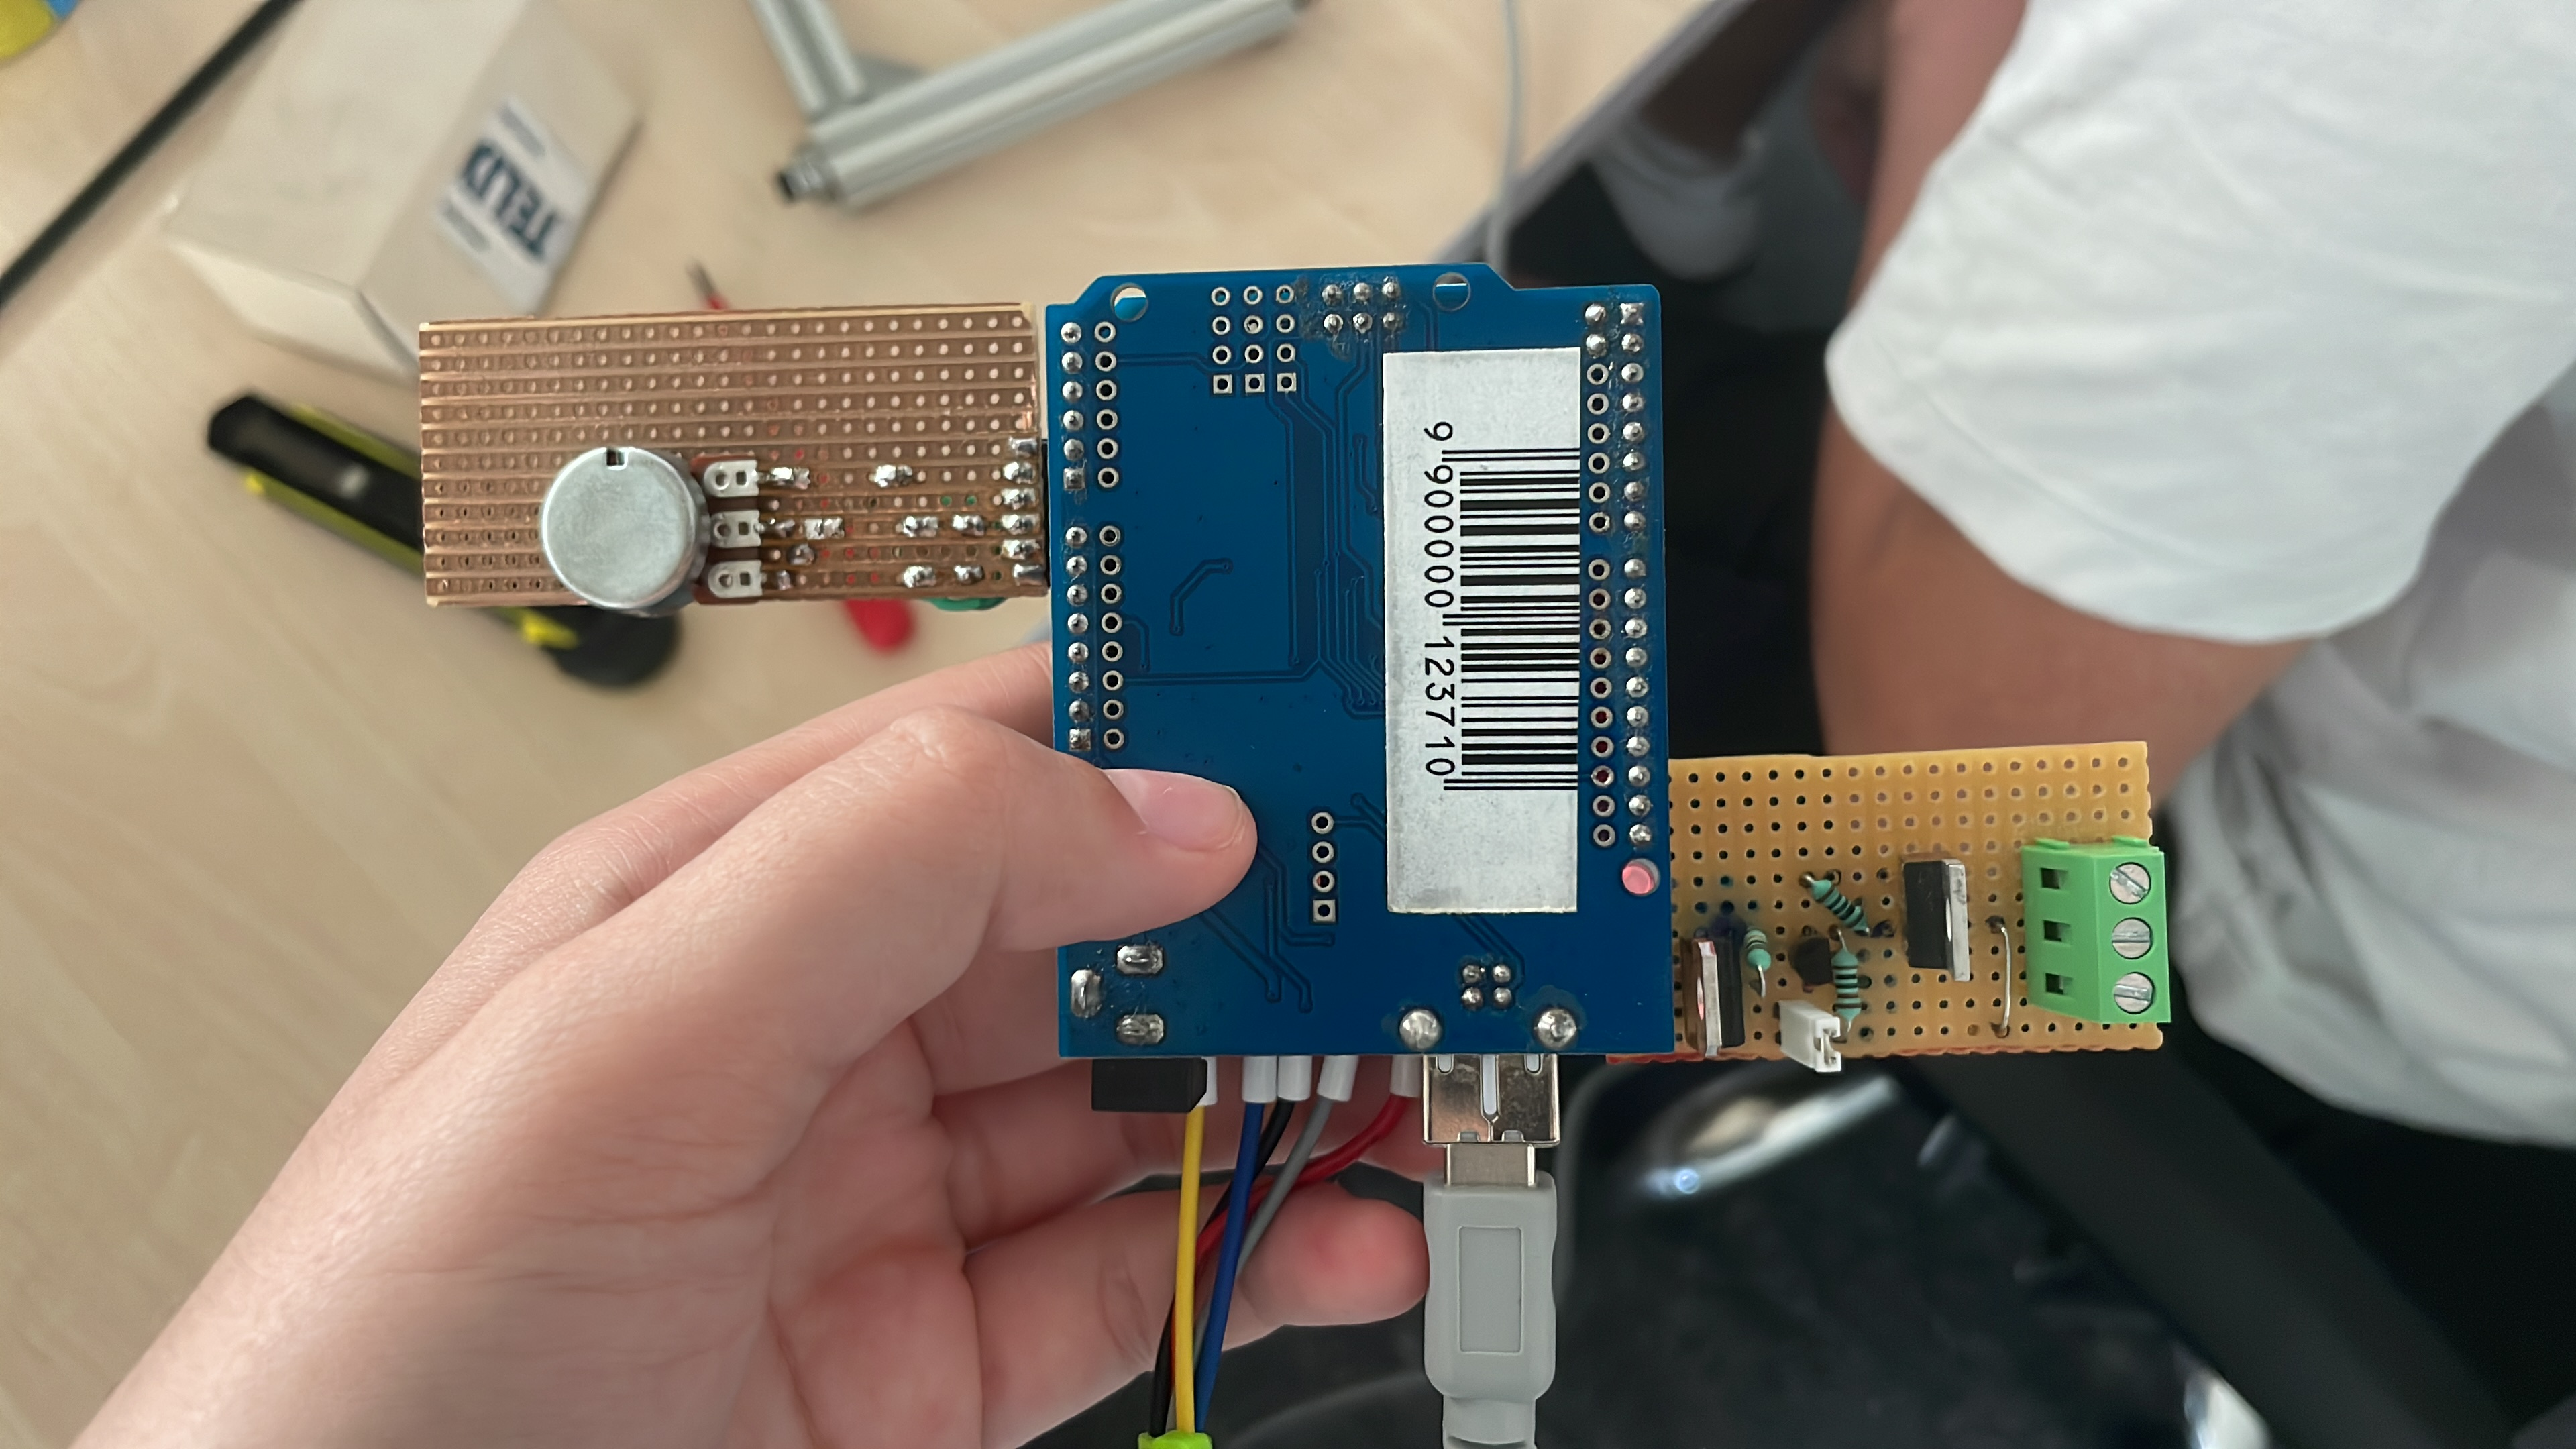
\includegraphics[angle = 270, width=0.75\linewidth]{backside.jpeg}
    \caption{Iza kontrolne table}
  \end{minipage}
\end{figure}


\newpage
\section{Skice motora}
\rhead{Skice motora}

Na slici 11 je prikazana osnovna i nepotpuna šema celog generatora. Desni četvorougao predstavlja kontrolnu kutiju, dok levi četvorougao predstavlja kontrolnu pločicu koja sadrži dugme i potenciometar kojim upravljamo motorom. 




\begin{figure}[htbp]
    \centering
    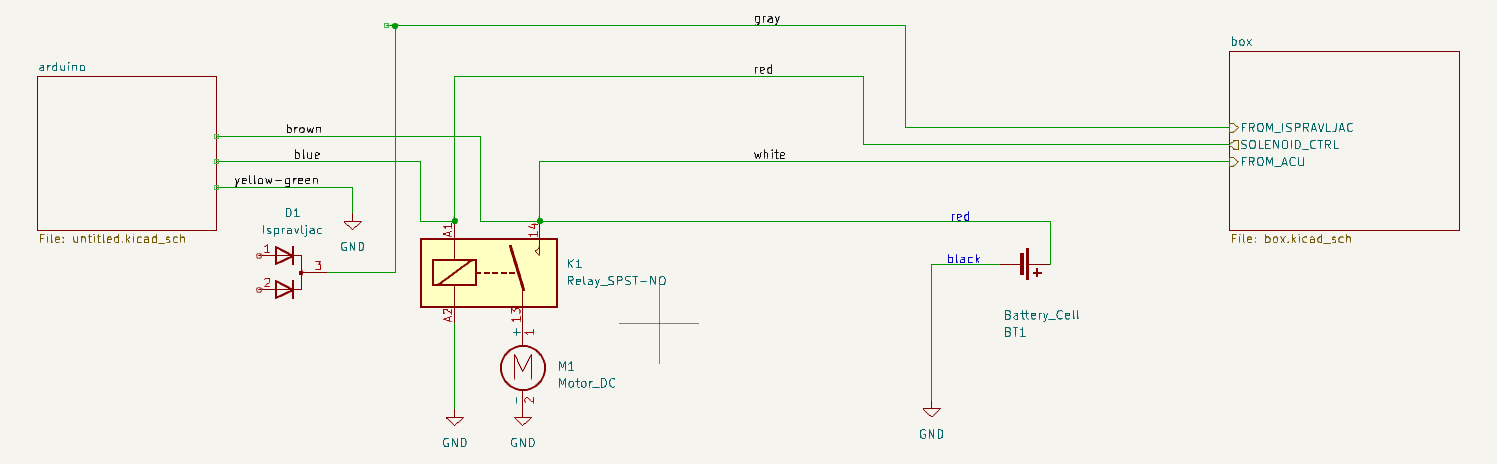
\includegraphics[width=1\linewidth]{skica_motor.png}
    \caption{Skica motora}
\end{figure}
Detalje kontrolne kutije možemo videti na slici 12 i u nastavku teksta. 



\begin{figure}[htbp]
    \centering
    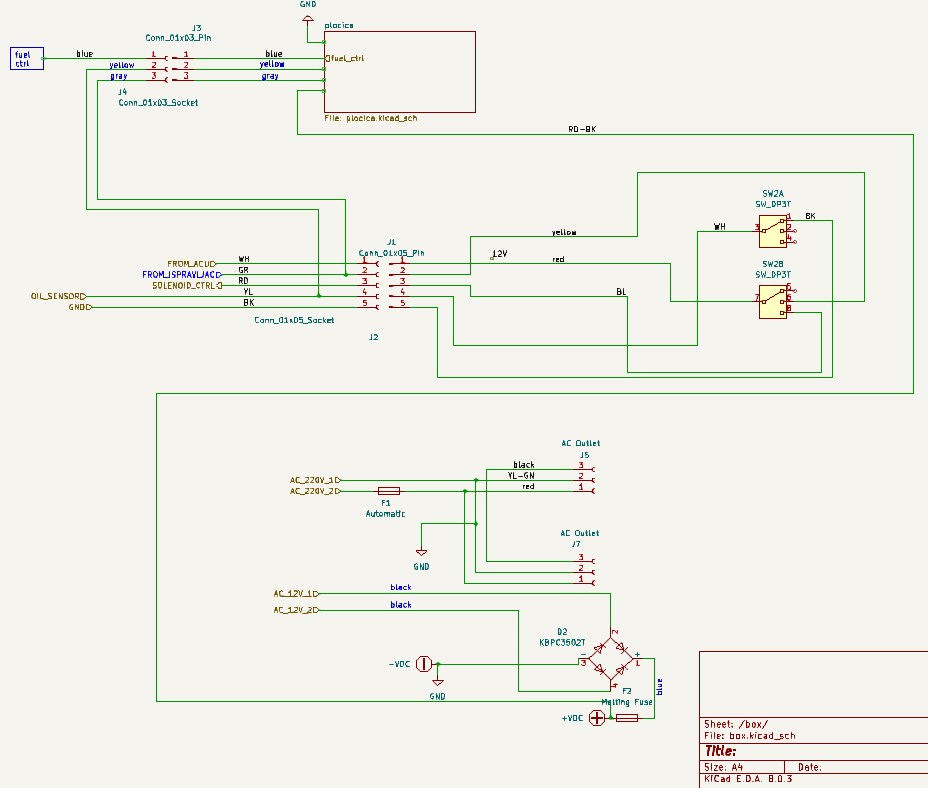
\includegraphics[width=0.75\linewidth]{elektronika.png}
    \caption{Skica elektronike}
\end{figure}

Šema kontrolne table jasno prikazuje način na koji su sve komponente povezane unutar kontrolne table kao i komponente van nje. \\

Kontrolna tabla prima signale sa ispravljača, senzora za ulje kao i izlaznu struju generatora. Iz table izlazni signal prema generatoru je kontrola solenoida koja služi za pokretanje motora na pritisak tastera ili okretom ključa. Na prednjoj strani panela nalaze se dve AC utičnice, kao i DC izlaz. \\

Iza kontrolne table, u kutiji, pored svega toga nalaze se dodatne komponente poput mosta, osigurača i pločice koja obrađuje signal ključa. \\




\begin{figure}[htbp]
    \centering
    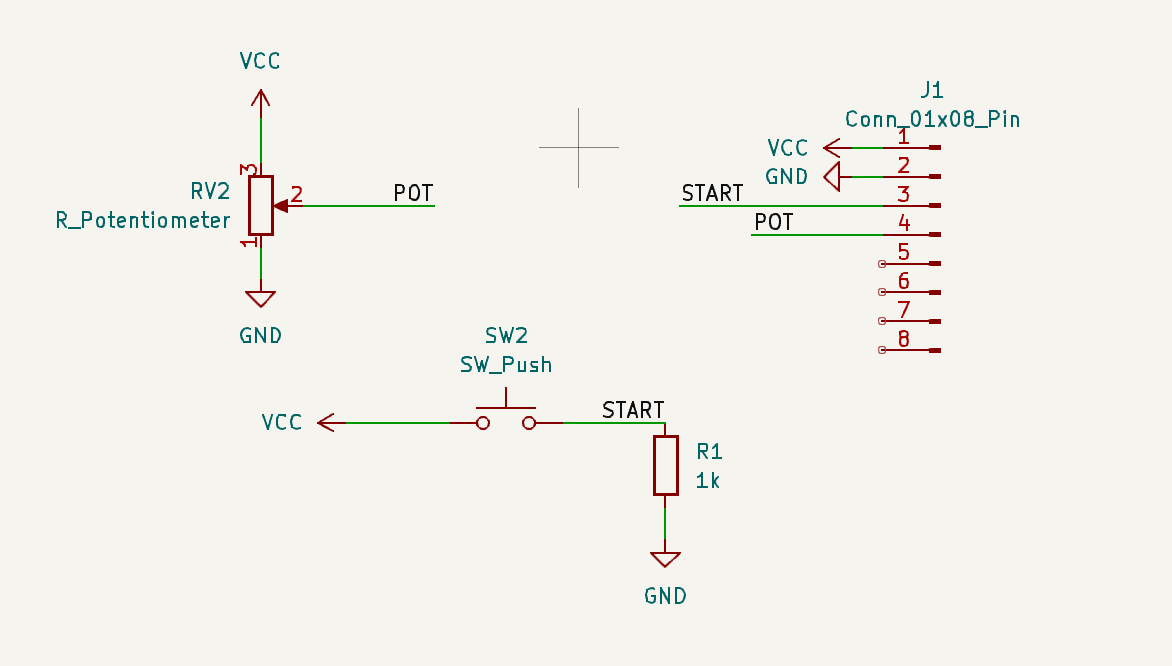
\includegraphics[width=1\linewidth]{kontrolna_plocica.png}
    \caption{Skica motora}
\end{figure}
Detalje kontrolne kutije možemo videti na slici 12 i u nastavku teksta. 



\begin{figure}[htbp]
    \centering
    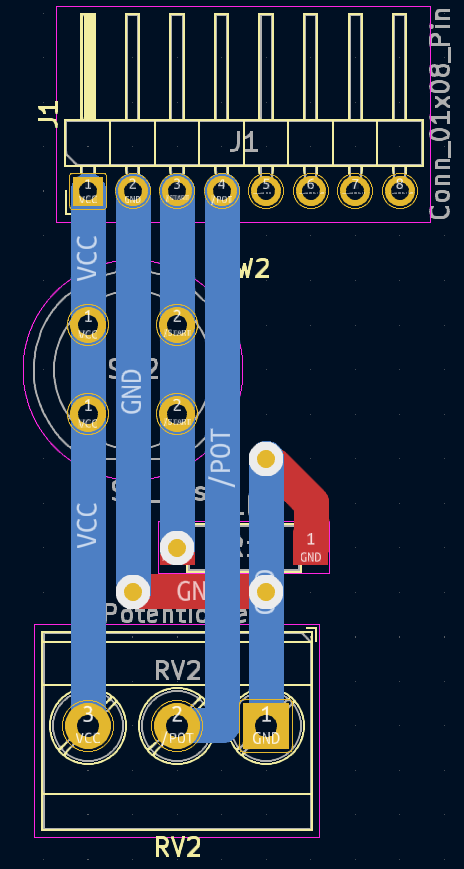
\includegraphics[angle = 270, width=0.8\linewidth]{pcb_plocice.png}
    \caption{Skica elektronike}
\end{figure}


Za sam kraj, na slikama 13 i 14 možemo videti šemu i pcb pločice koju smo napravili za kontrolu motora, koja sadrži dugme i potenciometar. 


\newpage
\section{Pokretanje motora}
\rhead{Pokretanje motora}

Ključ mora biti u kontaktu, okrene se potenciometar da menjač dođe u odgovarajući položaj (žuta sekcija \textit{SLOW}) i pritiskom na dugme palimo motor. 

\subsection{Firmwarwe za pločicu}

Signal sa dugmeta očitavamo sa analognog pina A0, prosleđuje se na pin 10 koji je povezan na solenoid, a \textit{stepper} je povezan na prvi \textit{stepper port} \textit{shield}-a za kontrolu motora pomoću arduina. 
Stanje potenciometra očitavamo sa analognog pina A3, i on pokreće \textit{stepper} motor upotrebom AdaFruits biblioteke. \\

Bazična podešavanja motora su sledeća: 
\begin{itemize}
\item STEP(60) - ugaoni pomeraj
    \item MOTORSPEED(48) - brzina motora
\end{itemize}

Na početku programa pravi se objekat klase \textit{AF\_Stepper}. Brzinu mu postavljamo metodom \textbf{setSpeed}. U zavisnosti od trenutnog stanja potenciometra, motor se pomera u smeru kazaljke na satu ili obrnuto pomoću metode \textbf{step}, uz parametar \textit{FORWARDS/BACKWARDS}. Pri završetku kretanja metoda \textbf{release} opušta motor, sklanja pritisak sa njega i smanjuje temperaturu, čime sprečava pregrejavanje.



\newpage
\section{Potrebni linkovi}
\rhead{Potrebni linkovi}

Link za AdaFruits \href{https://github.com/adafruit/Adafruit_Motor-Shield-v1}{GitHub repozitorijum}, kao i za \href{https://learn.adafruit.com/adafruit-motor-shield/overview}{zvanični sajt}. 

Link našeg \href{https://youtube.com/shorts/waznABaG0Z0?feature=share}{YouTube videa} koji prikazuje rad motora kao i \href{https://github.com/antovic/LPRS2_2024/tree/main/Automotive/Diesel_Generator}{GitHub repozitorijuma}.



\end{document}
